%%%%%%%%%%%%%%%%%%%%%%%%%%%%%%%%%%%%%%%%%%%%%%%%%%%%%%%%%%%%%%%%%%%%%
%
% CSCI 1430 Writeup Template
%
% This is a LaTeX document. LaTeX is a markup language for producing
% documents. Your task is to fill out this
% document, then to compile this into a PDF document.
%
% TO COMPILE:
% > pdflatex thisfile.tex
%
% For references to appear correctly instead of as '??', you must run
% pdflatex twice.
%
% If you do not have LaTeX and need a LaTeX distribution:
% - Departmental machines have one installed.
% - Personal laptops (all common OS): www.latex-project.org/get/
%
% If you need help with LaTeX, please come to office hours.
% Or, there is plenty of help online:
% https://en.wikibooks.org/wiki/LaTeX
%
% Good luck!
% James and the 1430 staff
%
%%%%%%%%%%%%%%%%%%%%%%%%%%%%%%%%%%%%%%%%%%%%%%%%%%%%%%%%%%%%%%%%%%%%%
%
% How to include two graphics on the same line:
%
% \includegraphics[\width=0.49\linewidth]{yourgraphic1.png}
% \includegraphics[\width=0.49\linewidth]{yourgraphic2.png}
%
% How to include equations:
%
% \begin{equation}
% y = mx+c
% \end{equation}
%
%%%%%%%%%%%%%%%%%%%%%%%%%%%%%%%%%%%%%%%%%%%%%%%%%%%%%%%%%%%%%%%%%%%%%%%%%%%%%%%%%%%%%%%%%%%%%%%%

\documentclass[11pt]{article}

\usepackage[english]{babel}
\usepackage[utf8]{inputenc}
\usepackage[colorlinks = true,
            linkcolor = blue,
            urlcolor  = blue]{hyperref}
\usepackage[a4paper,margin=1.5in]{geometry}
\usepackage{stackengine,graphicx}
\usepackage{fancyhdr}
\setlength{\headheight}{15pt}
\usepackage{microtype}
\usepackage{times}
\usepackage{booktabs}
\usepackage{float}

% python code format: https://github.com/olivierverdier/python-latex-highlighting
\usepackage{pythonhighlight}

\frenchspacing
\setlength{\parindent}{0cm} % Default is 15pt.
\setlength{\parskip}{0.3cm plus1mm minus1mm}

\pagestyle{fancy}
\fancyhf{}
\lhead{Homework 5 Writeup}
\rhead{CSCI 1430}
\rfoot{\thepage}

\date{}

\title{\vspace{-1cm}Homework 5 Writeup}


\begin{document}
\maketitle
\vspace{-2cm}
\thispagestyle{fancy}

\section*{Instructions}
\begin{itemize}
  \item Provide an overview about how your project functions. 
  \item Describe any interesting decisions you made to write your algorithm.
  \item Show and discuss the results of your algorithm.
  \item Feel free to include code snippets, images, and equations.
  \item List any extra credit implementation and result (optional).
  \item Use as many pages as you need, but err on the short side.
  \item \textbf{Please make this document anonymous.}
\end{itemize}

\section*{Project Overview}

This project is about training a convolutional neural network to perform scene
classification. We train a head on a pre-trained model, and create and train a
model from scratch.

\section*{Implementation Detail}

\section*{Result}

\begin{figure}[H]
    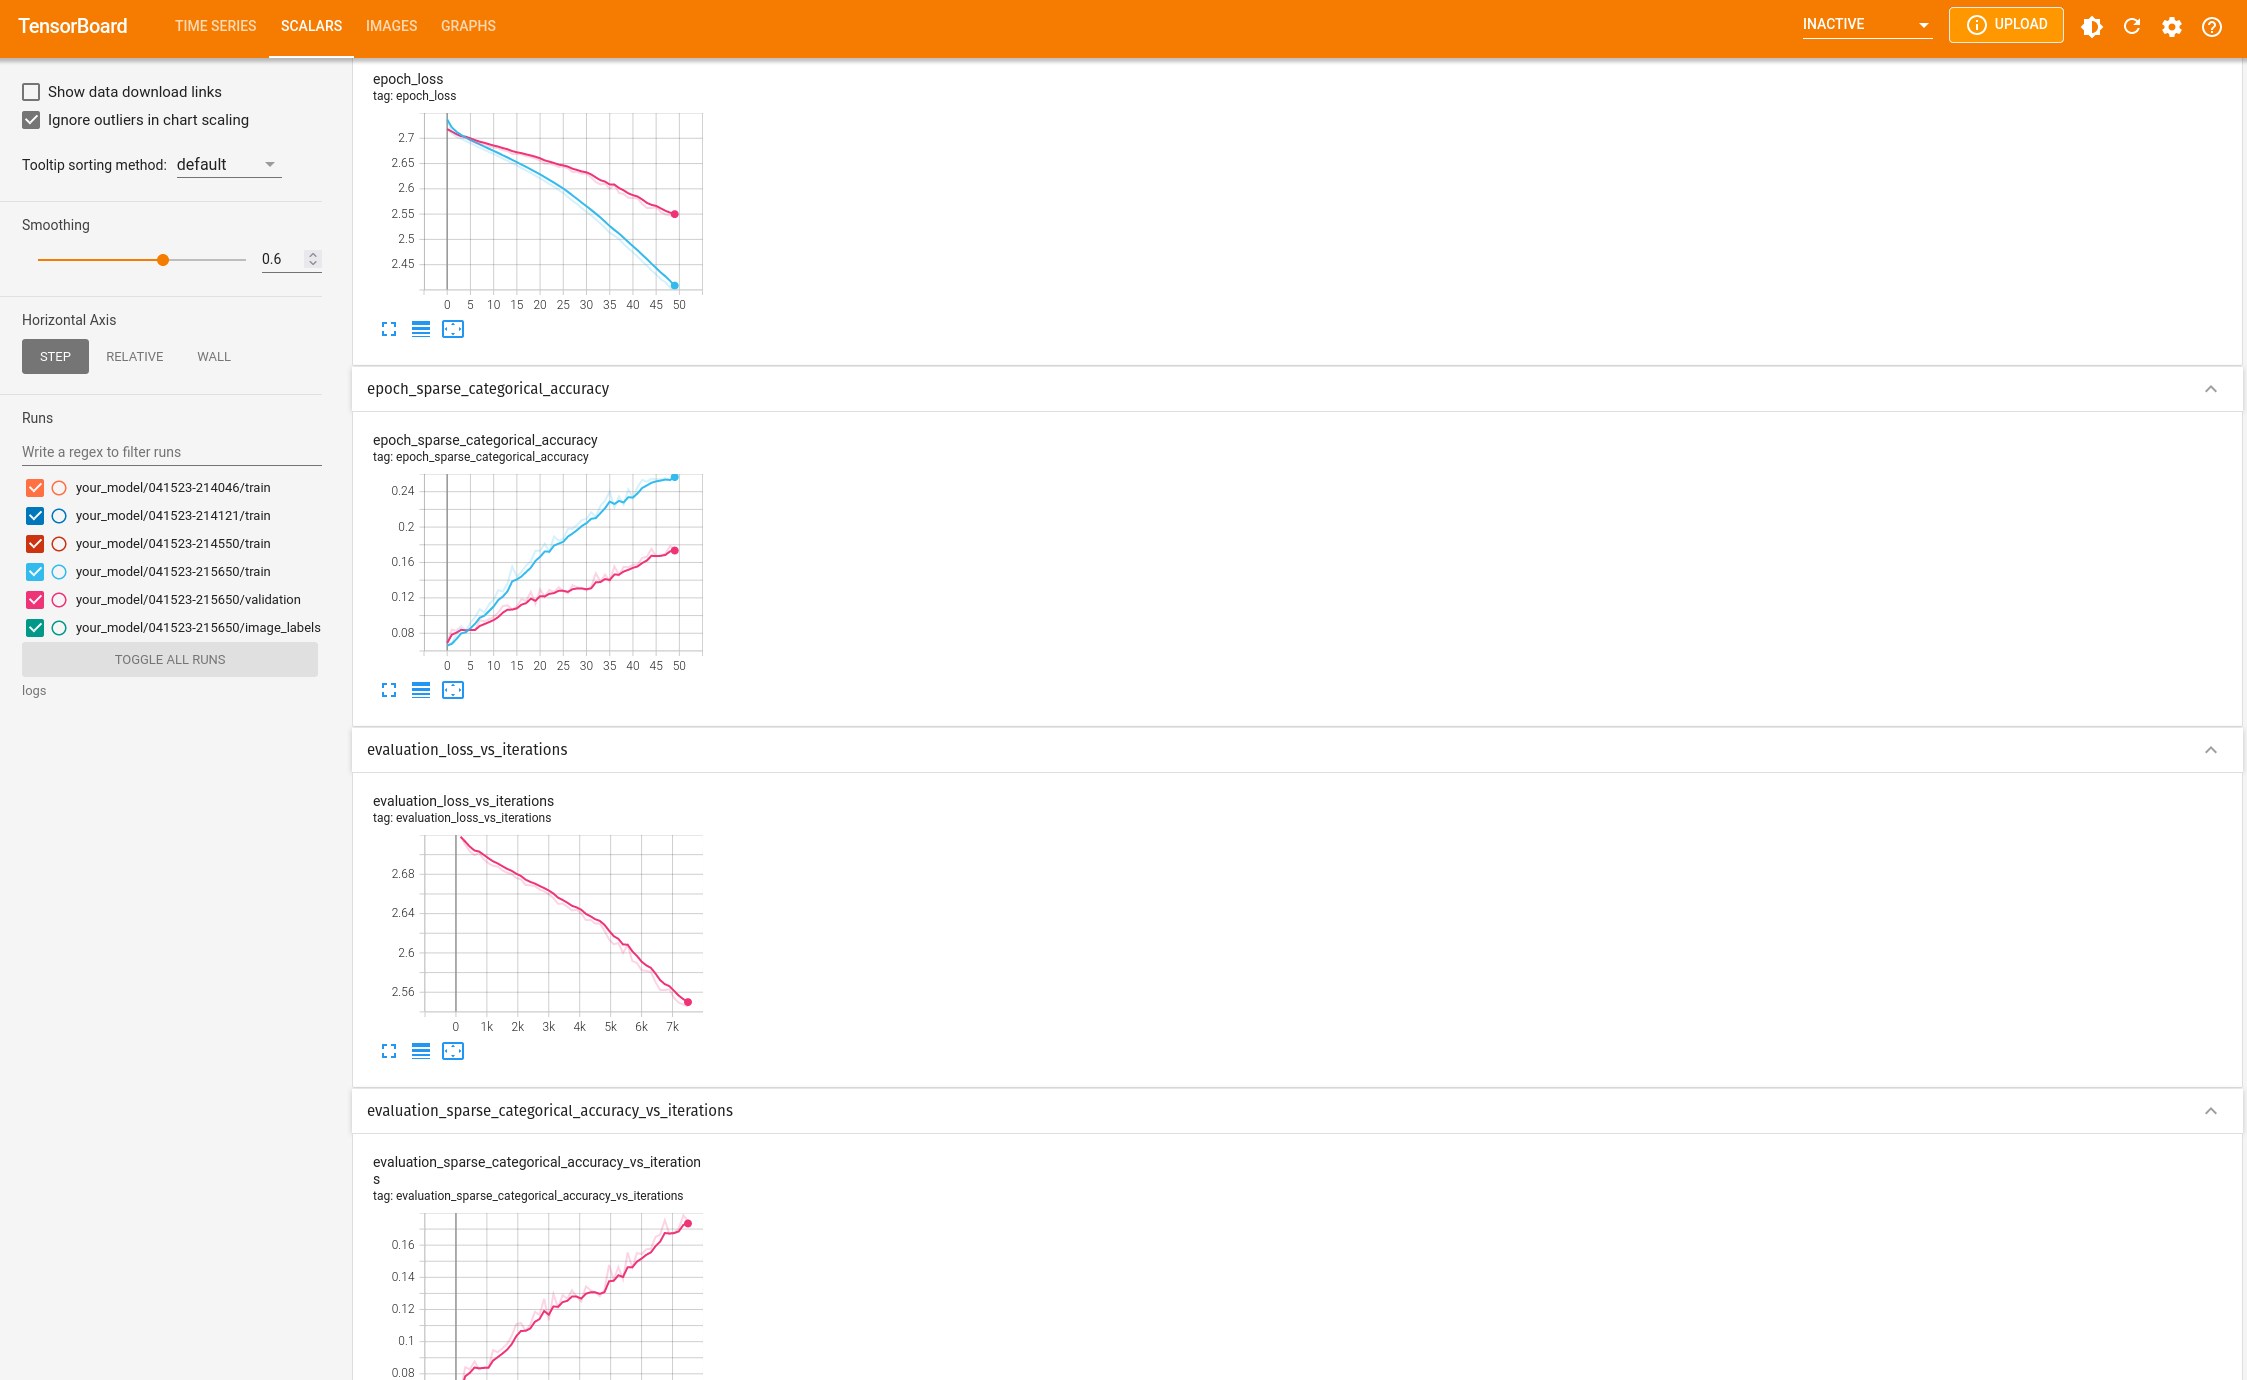
\includegraphics[width=10cm]{task1v0-2.png}
    \caption{Task 1:Training the small model on CPU. Somehow this was very fast.}
    \label{fig:result1}
\end{figure}

\begin{figure}[H]
    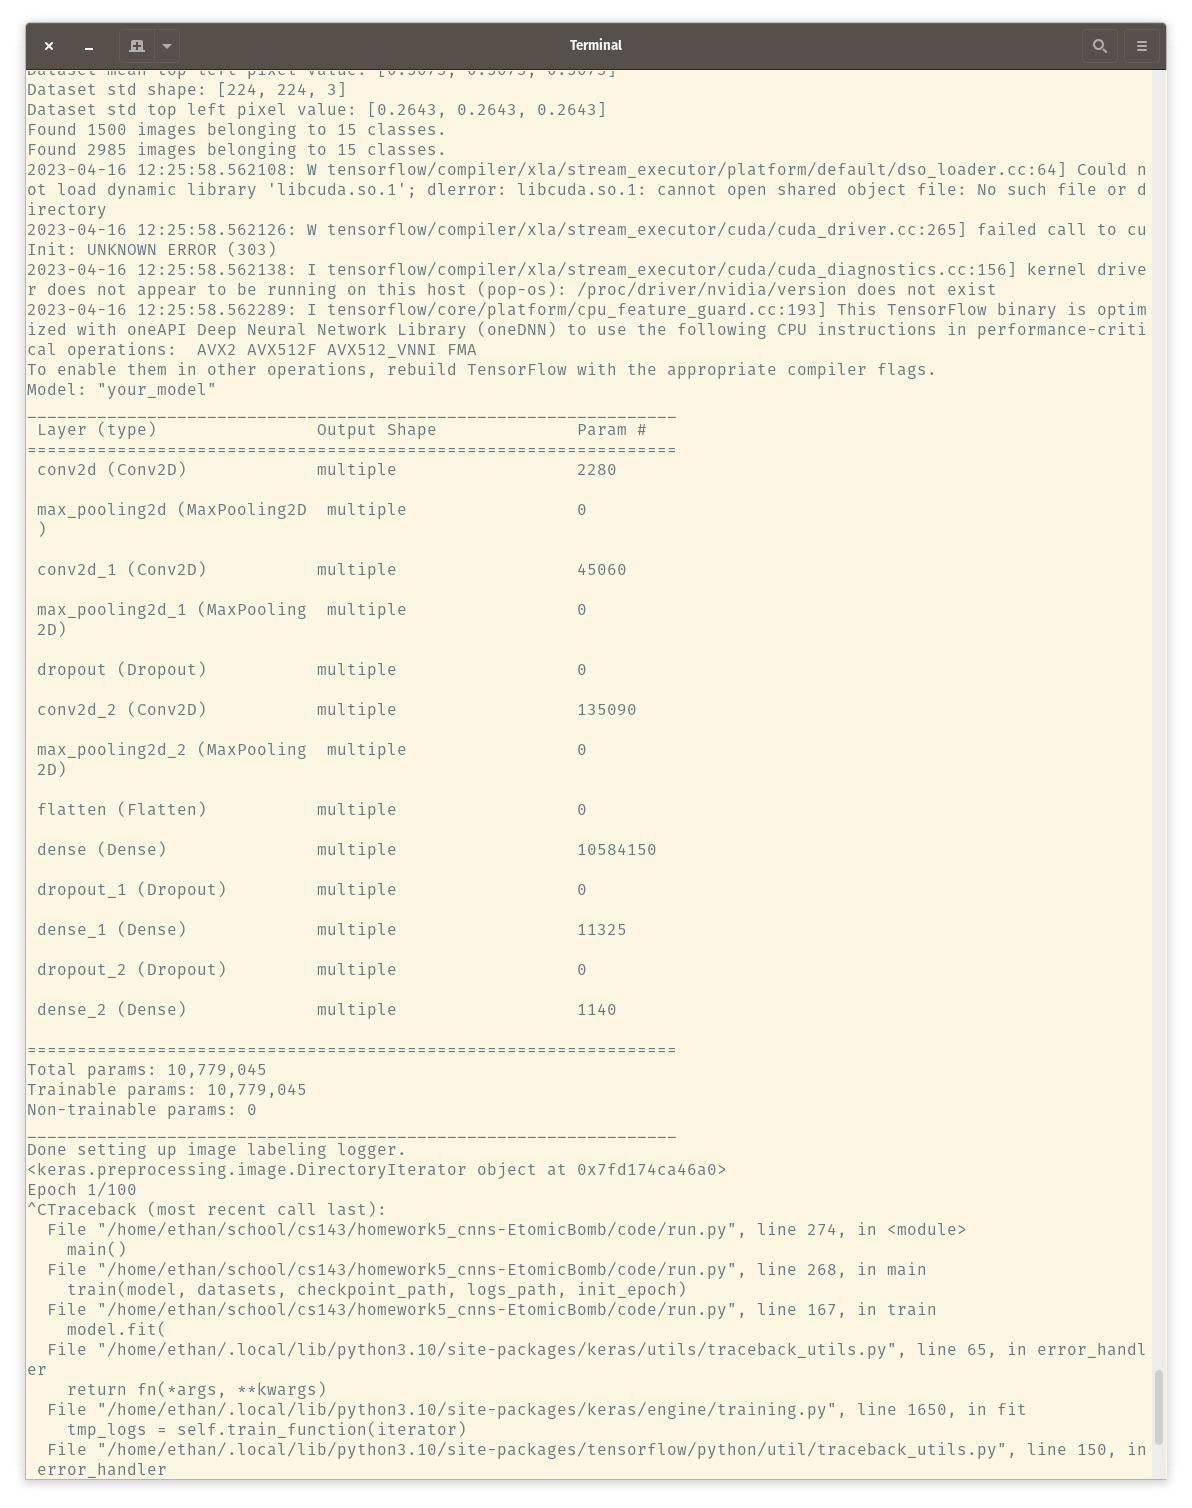
\includegraphics[width=10cm]{complete-parameters.png}
    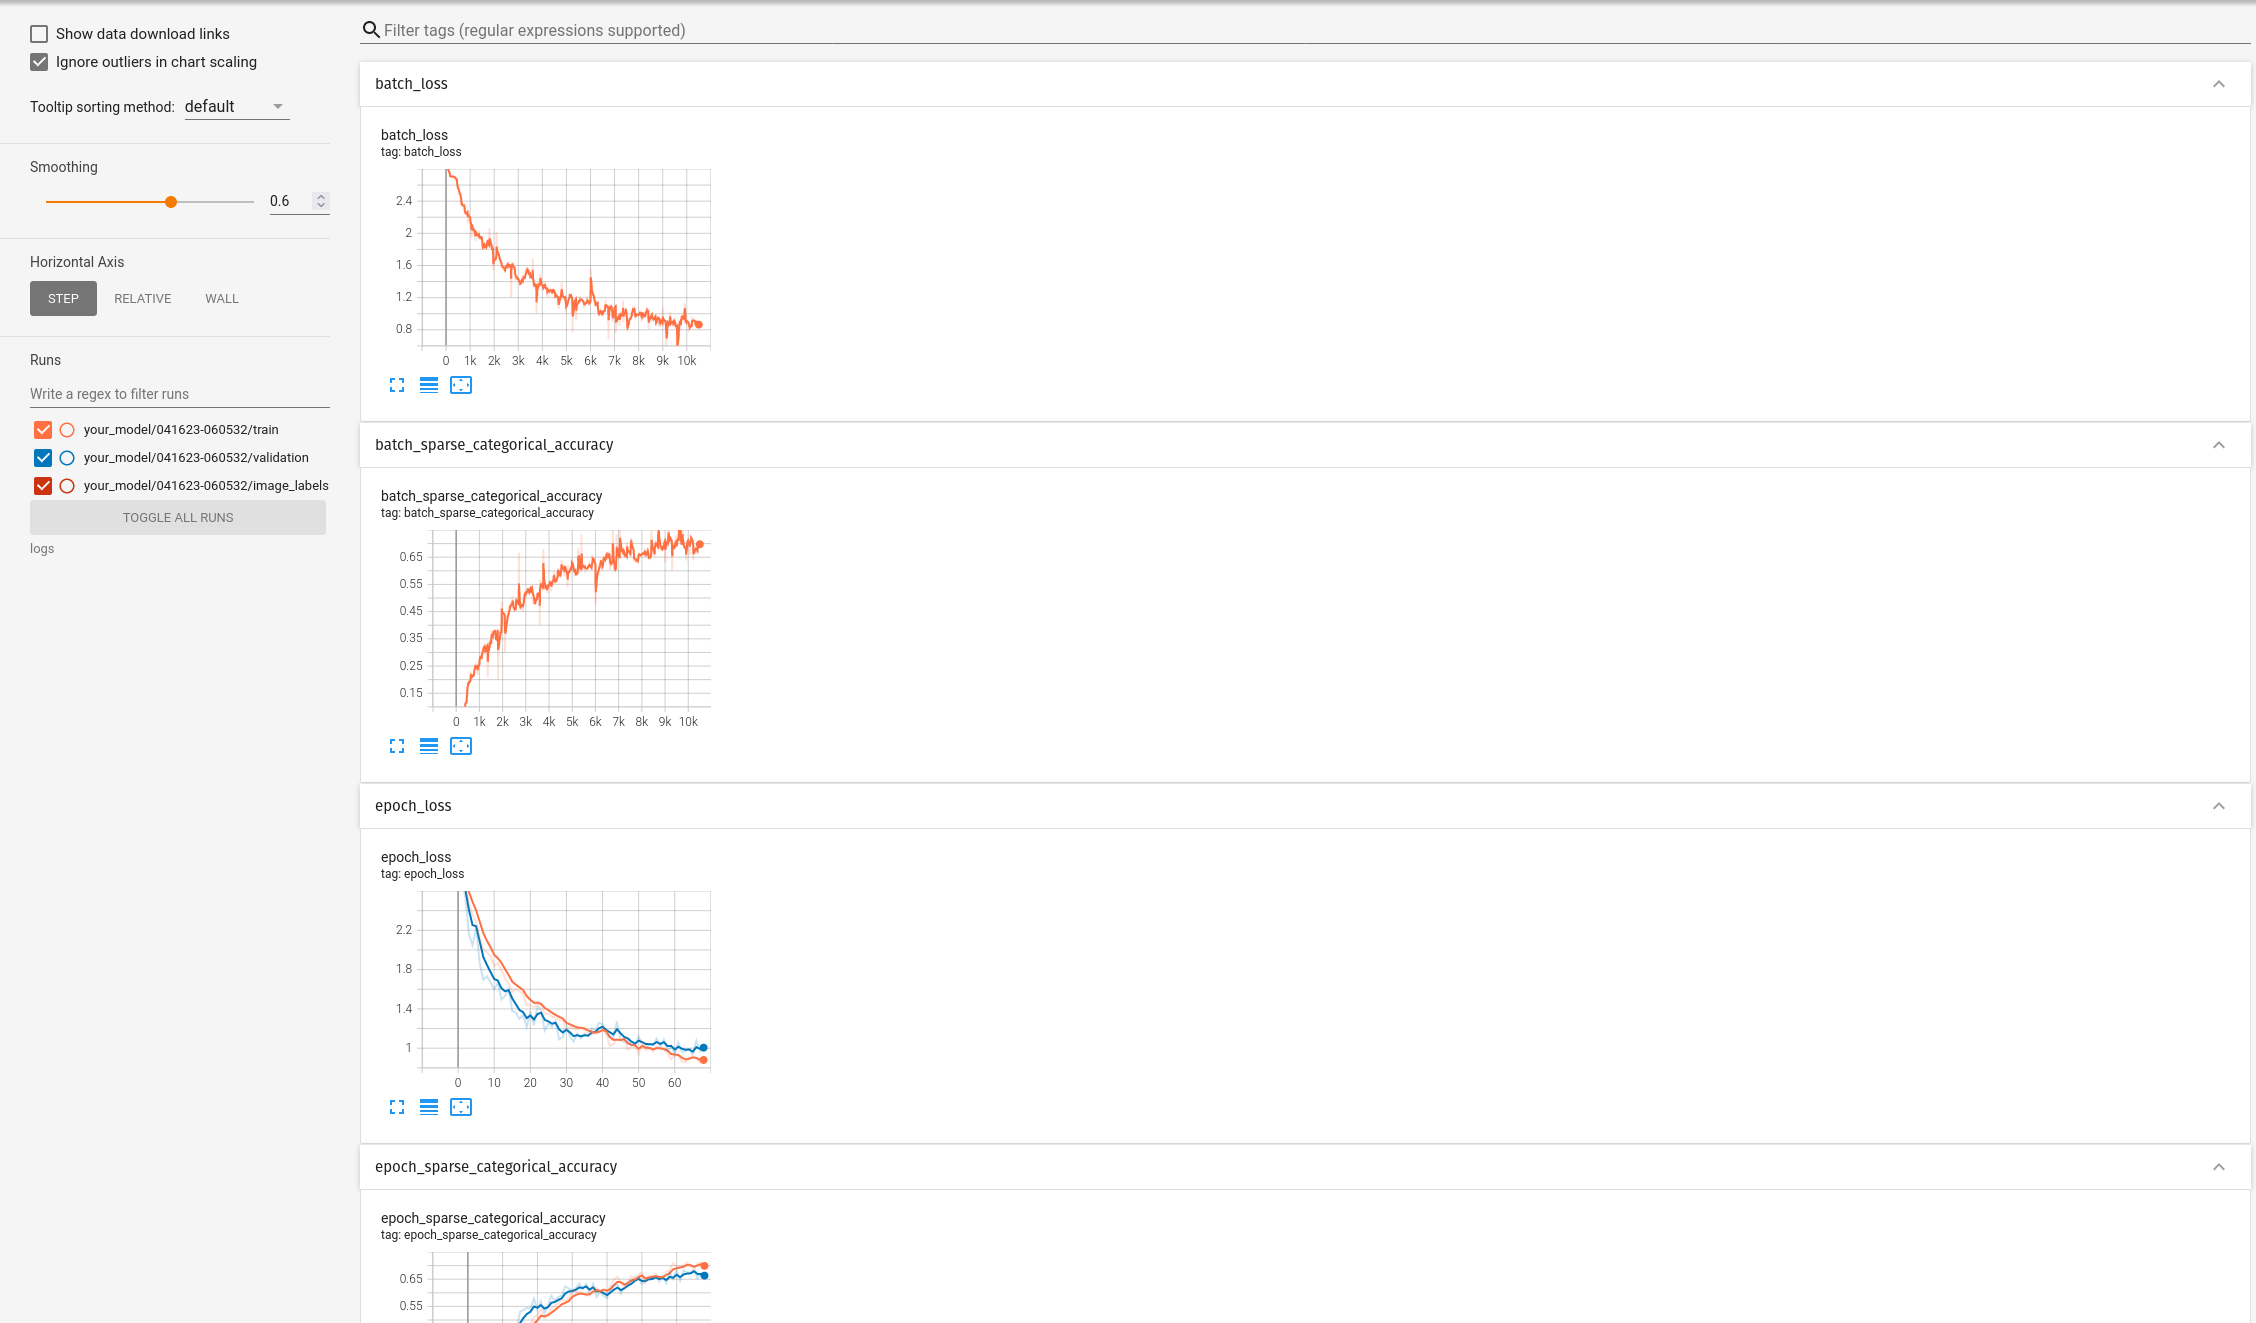
\includegraphics[width=10cm]{complete-a.png}
    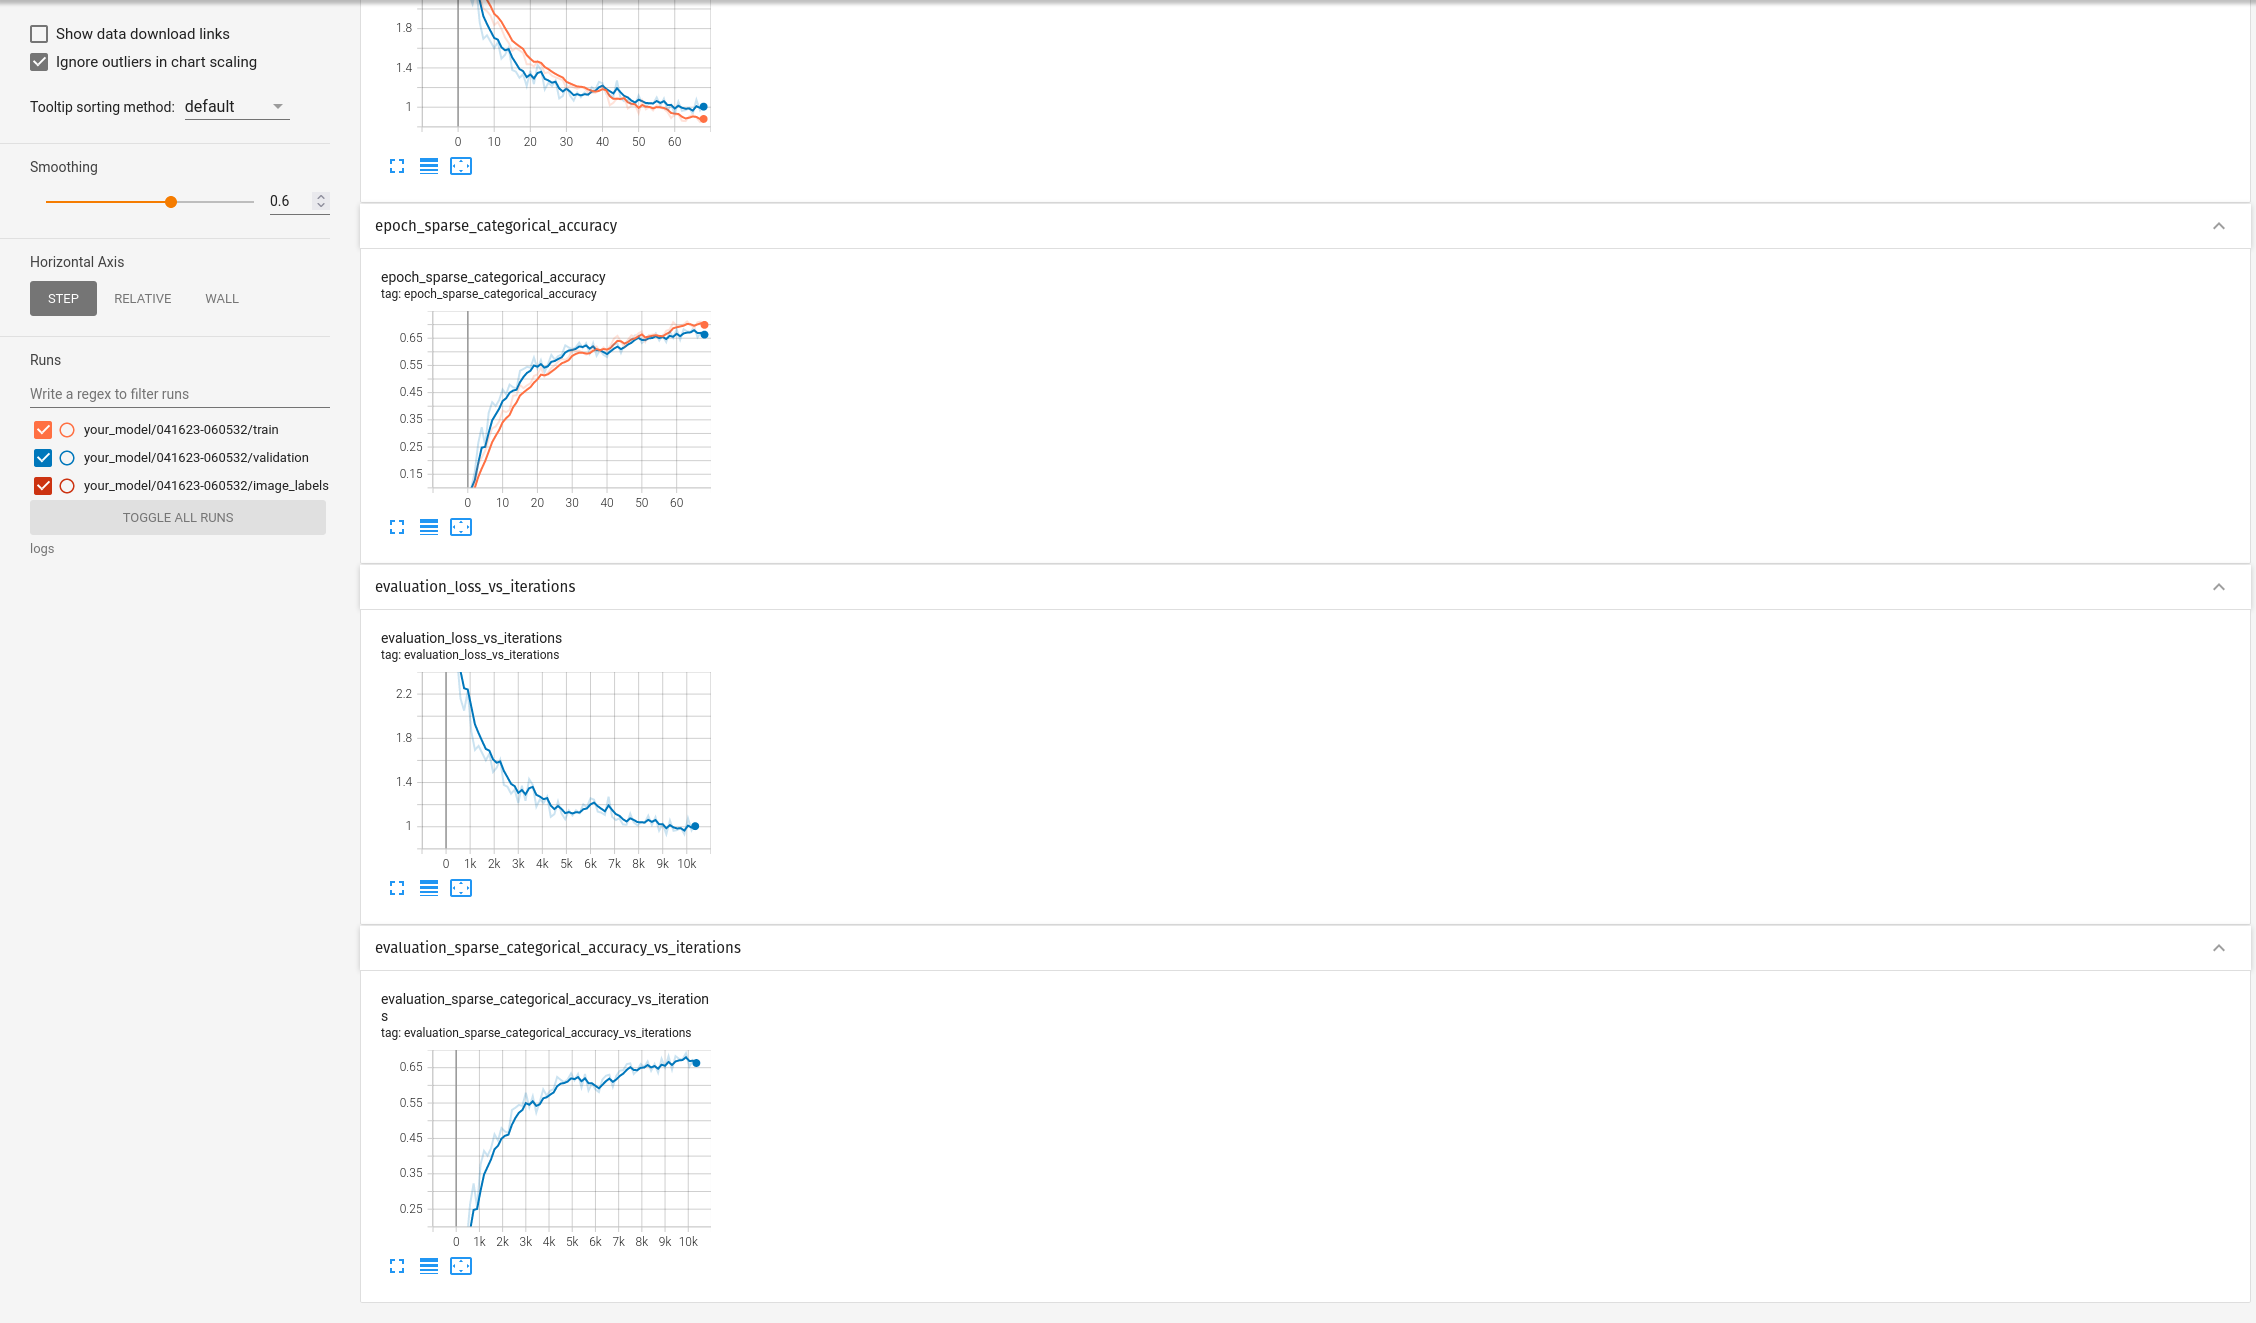
\includegraphics[width=10cm]{complete-b.png}
    \caption{Progress training the complete model}
    \label{fig:result1}
\end{figure}

% TODO: changes to performance after adding 

\begin{table}[H]
    \centering
    \begin{tabular}{lcr}
        \toprule
        With & Epochs & Sparse categorization accuracy \\
        \midrule
        Base & 3 & 0.2315 \\
        Standardization & 3& 0.1300 \\
        Data augmentation & 3 & 0.1008 \\
        Regularization & 56 & 0.6873 \\
        \bottomrule
    \end{tabular}
    \caption{Task 1 performance after adding each intermediate sophistication. 
I was able to train the network with full standardization, augmentation,
and regularization on Colab. The intermediate networks were trained on my laptop
(which only has a cpu -- thus limited epochs). This is because I was not able to
access Colab GPUs due to availability limits when I went back to do at the
intermediate stages.
I believe the decreasing accuracy as more sophistication was added is just
because of random chance and high variation from few epochs.
I noticed that before adding data augmentation (on my lost intermediate run, when I still
could use Colab) the training accuracy was able to get to basically 100, while
the test accuracy stayed low - maybe in the 20s or 30s. When I added
augmentation, the accuracy in training and testing coincided.}
    \label{tab:table1}
\end{table}

\begin{figure}[H]
    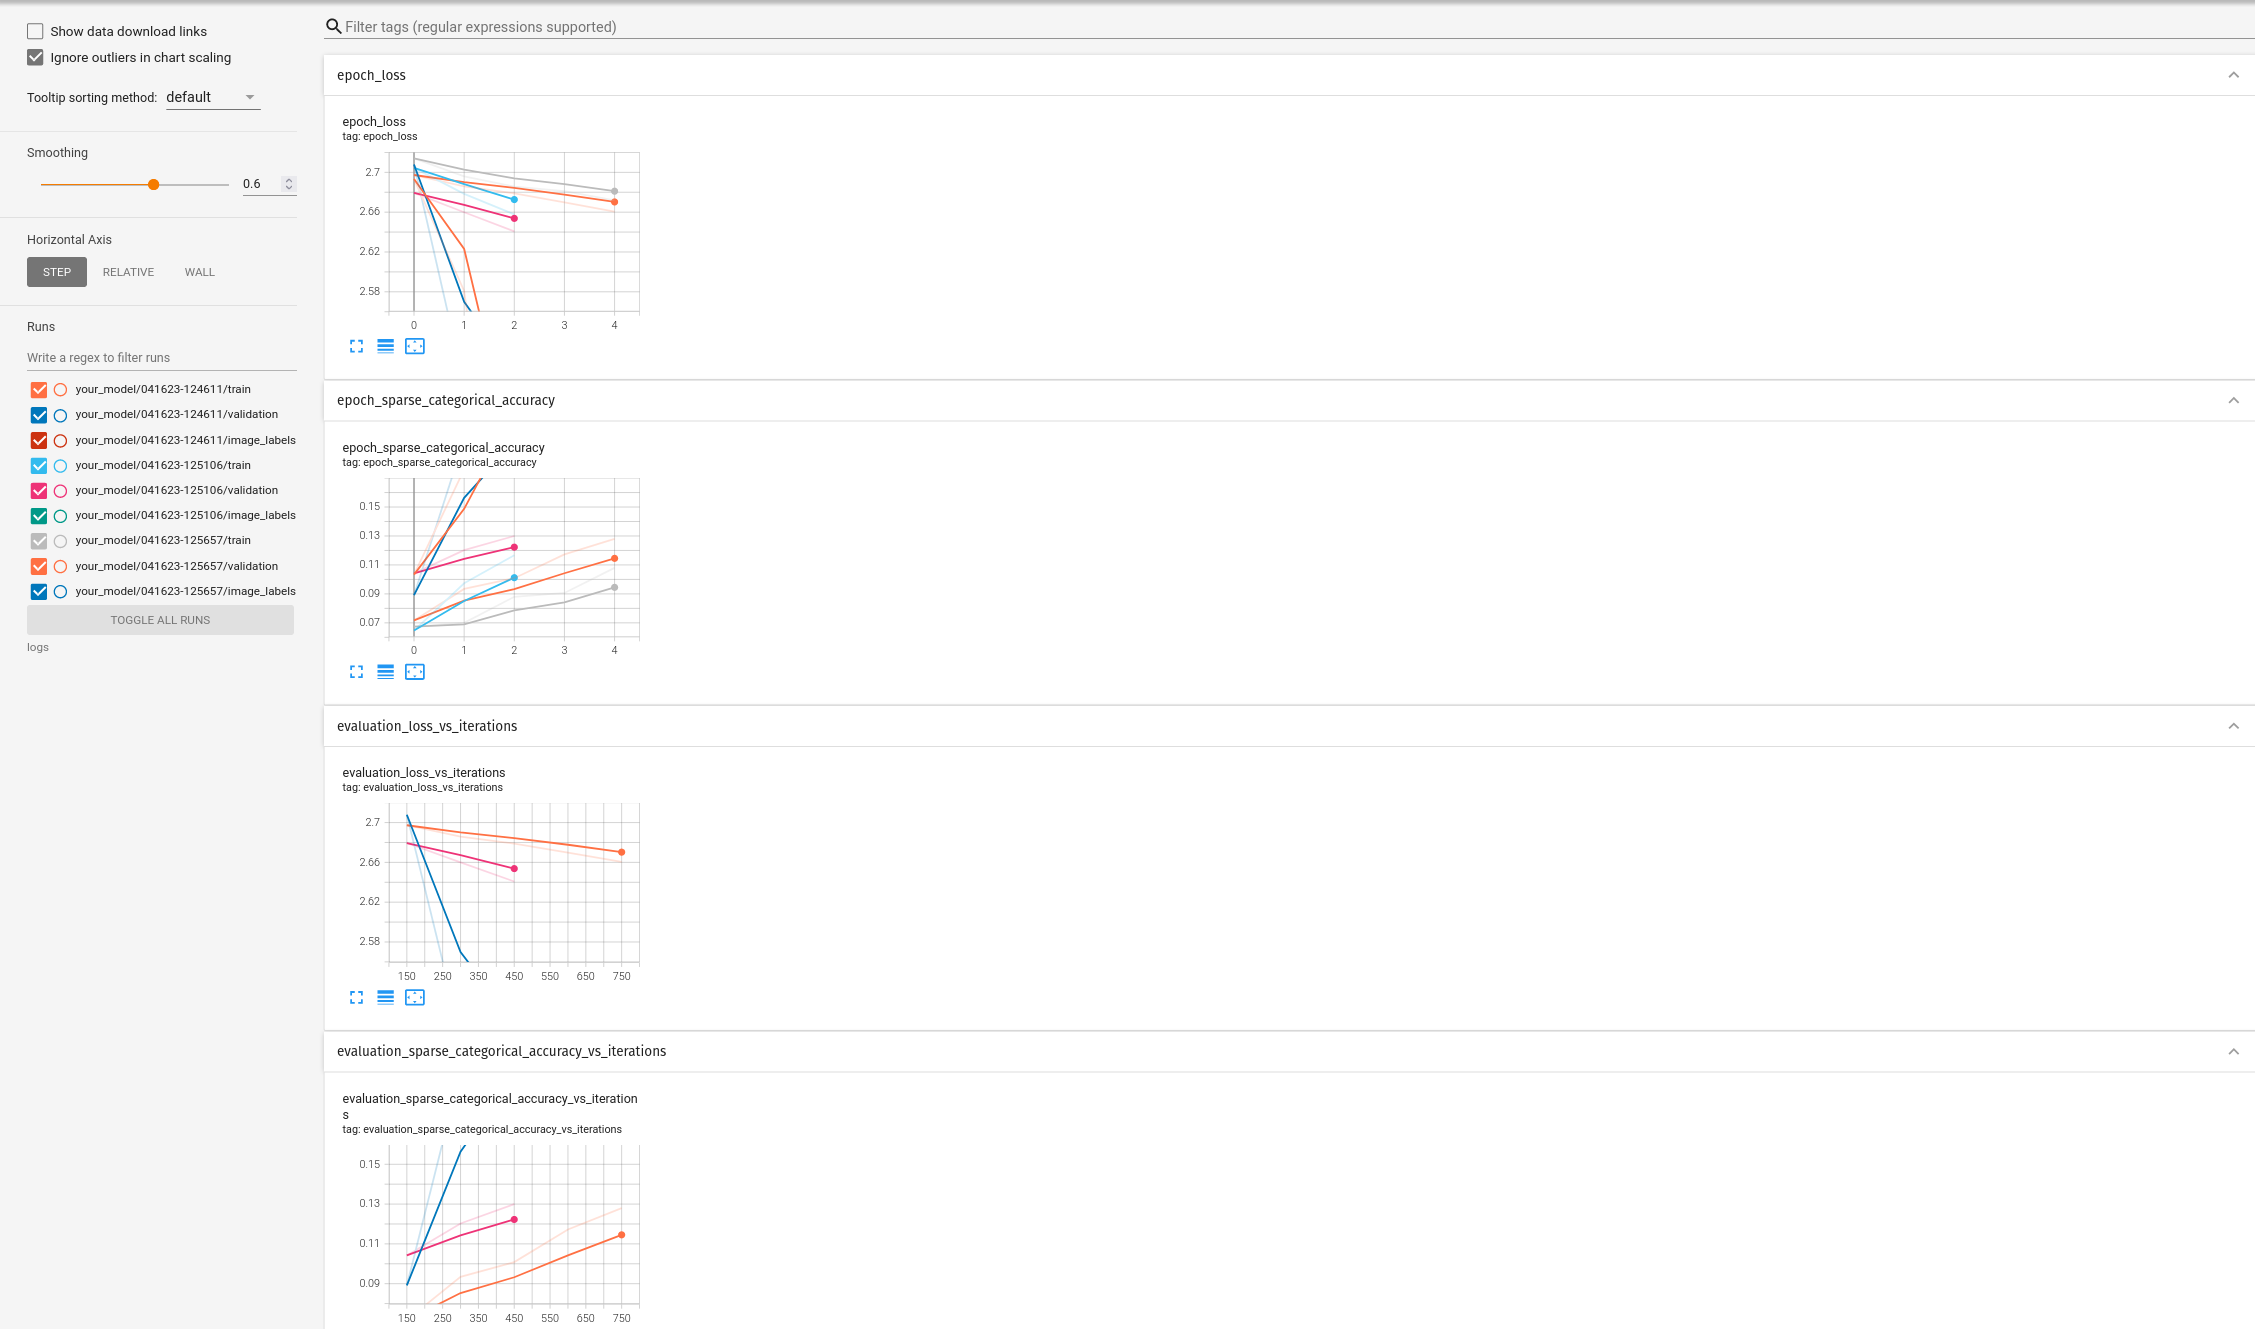
\includegraphics[width=10cm]{intermediate-cpu.png}
    \caption{Task 1: Progress training the intermediate models.}
    \label{fig:result1}
\end{figure}


\begin{table}[H]
    \centering
    \begin{tabular}{lr}
        \toprule
        Type & Sparse categorization accuracy \\
        \midrule
        Total & 0.9106 \\
        \bottomrule
    \end{tabular}
    \caption{Task 3 performance}
    \label{tab:table2}
\end{table}


\begin{figure}[H]
    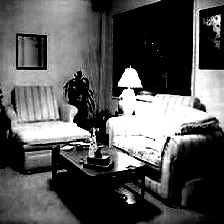
\includegraphics[width=7cm]{bedroom-should-living-room.png}
    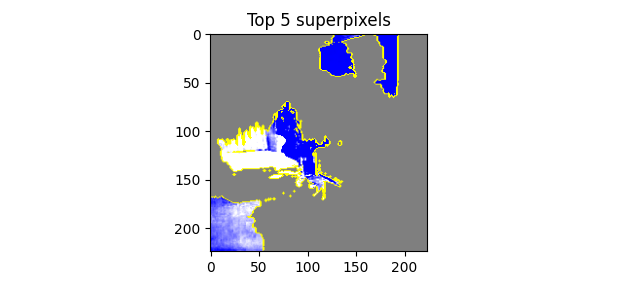
\includegraphics[width=7cm]{lime-bedroom-should-living-room.png}
    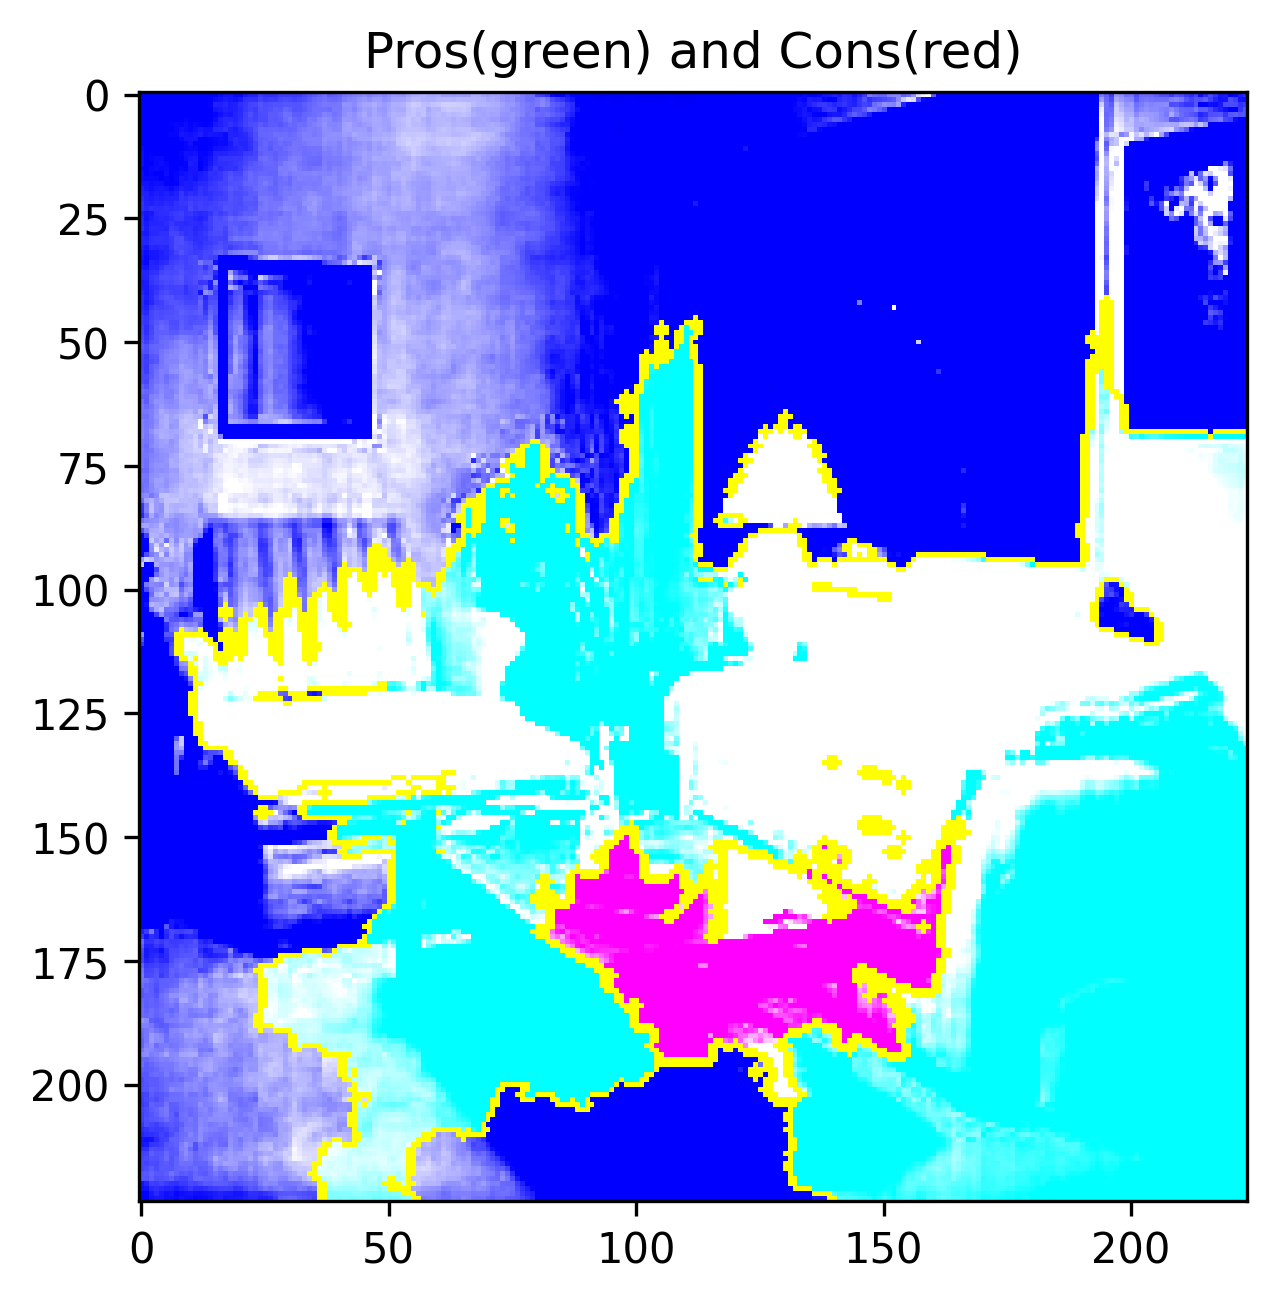
\includegraphics[width=7cm]{procon-bedroom-should-living-room.png}
    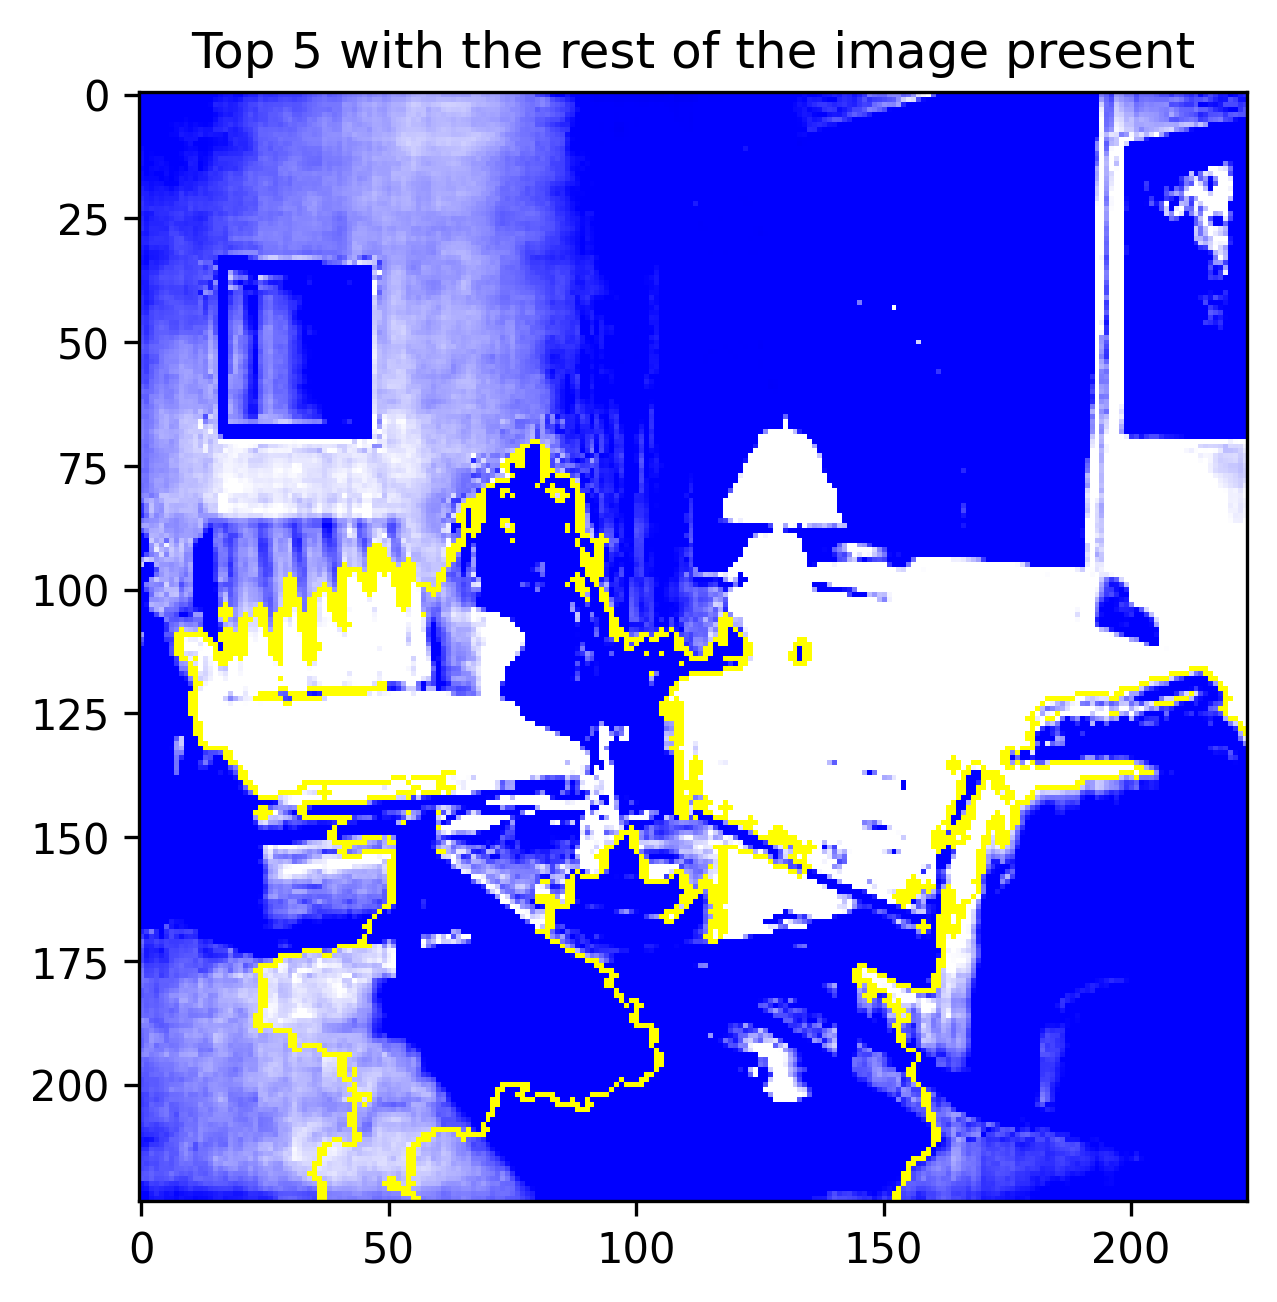
\includegraphics[width=7cm]{top5-bedroom-should-living-room.png}
    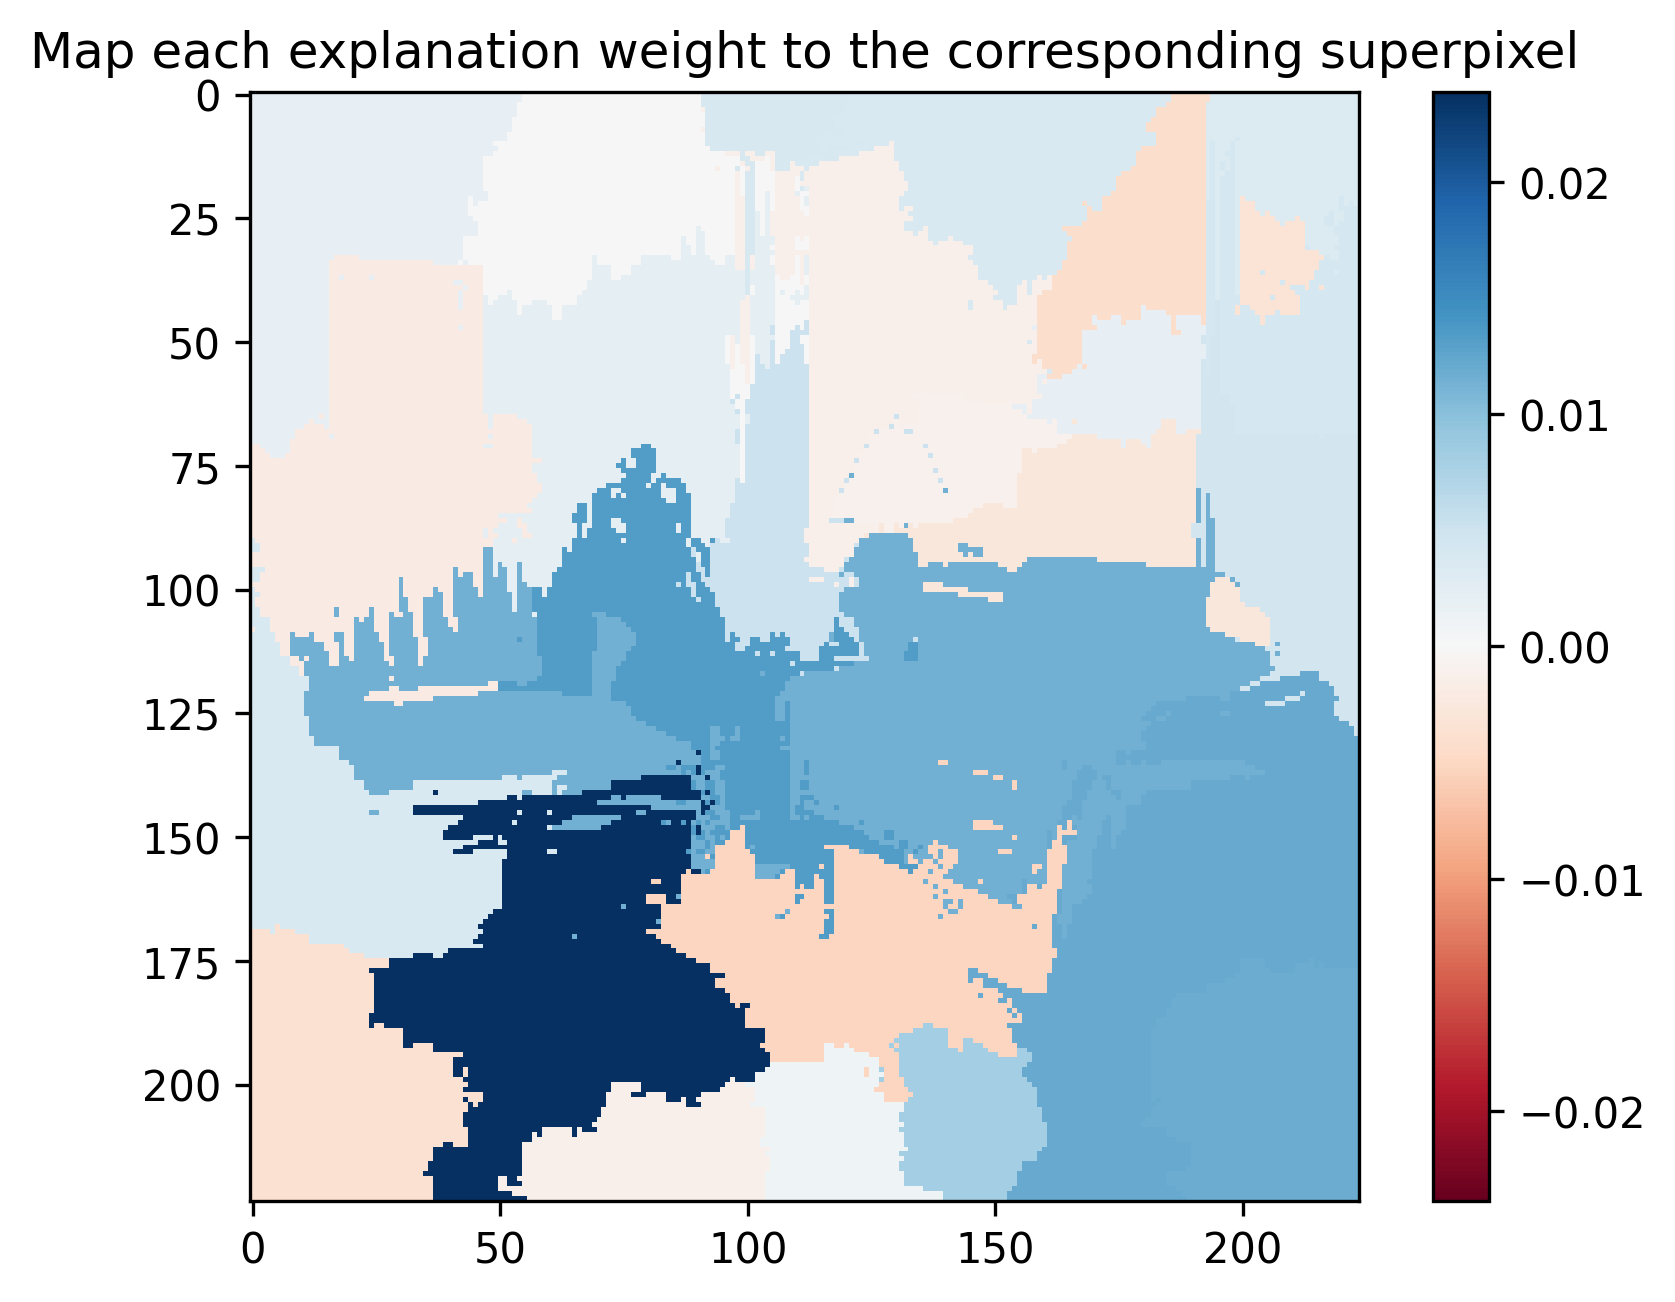
\includegraphics[width=7cm]{weight-bedroom-should-living-room.png}
    \caption{This is a bedroom, but was predicted as a living room.  Curious.
    This model seemed to focus on the middle left of the image, especially the
    floor and part of the chair. It also seemed to attend to the window. These
    features -- floors, chairs, and windows are all part of both bedrooms and living
    rooms. If it only attended to these features it's not suprising that it
    would get confused. I was not able to figure out whether it likes using the
    sky for its successful classifications.}
    \label{fig:result1}
\end{figure}

\begin{figure}[H]
    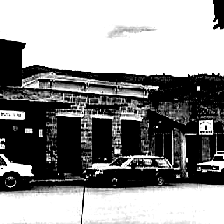
\includegraphics[width=7cm]{suburb-should-insidecity.png}
    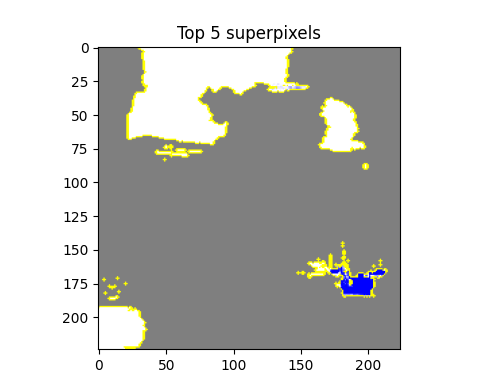
\includegraphics[width=7cm]{lime-suburb-should-insidecity.png}
    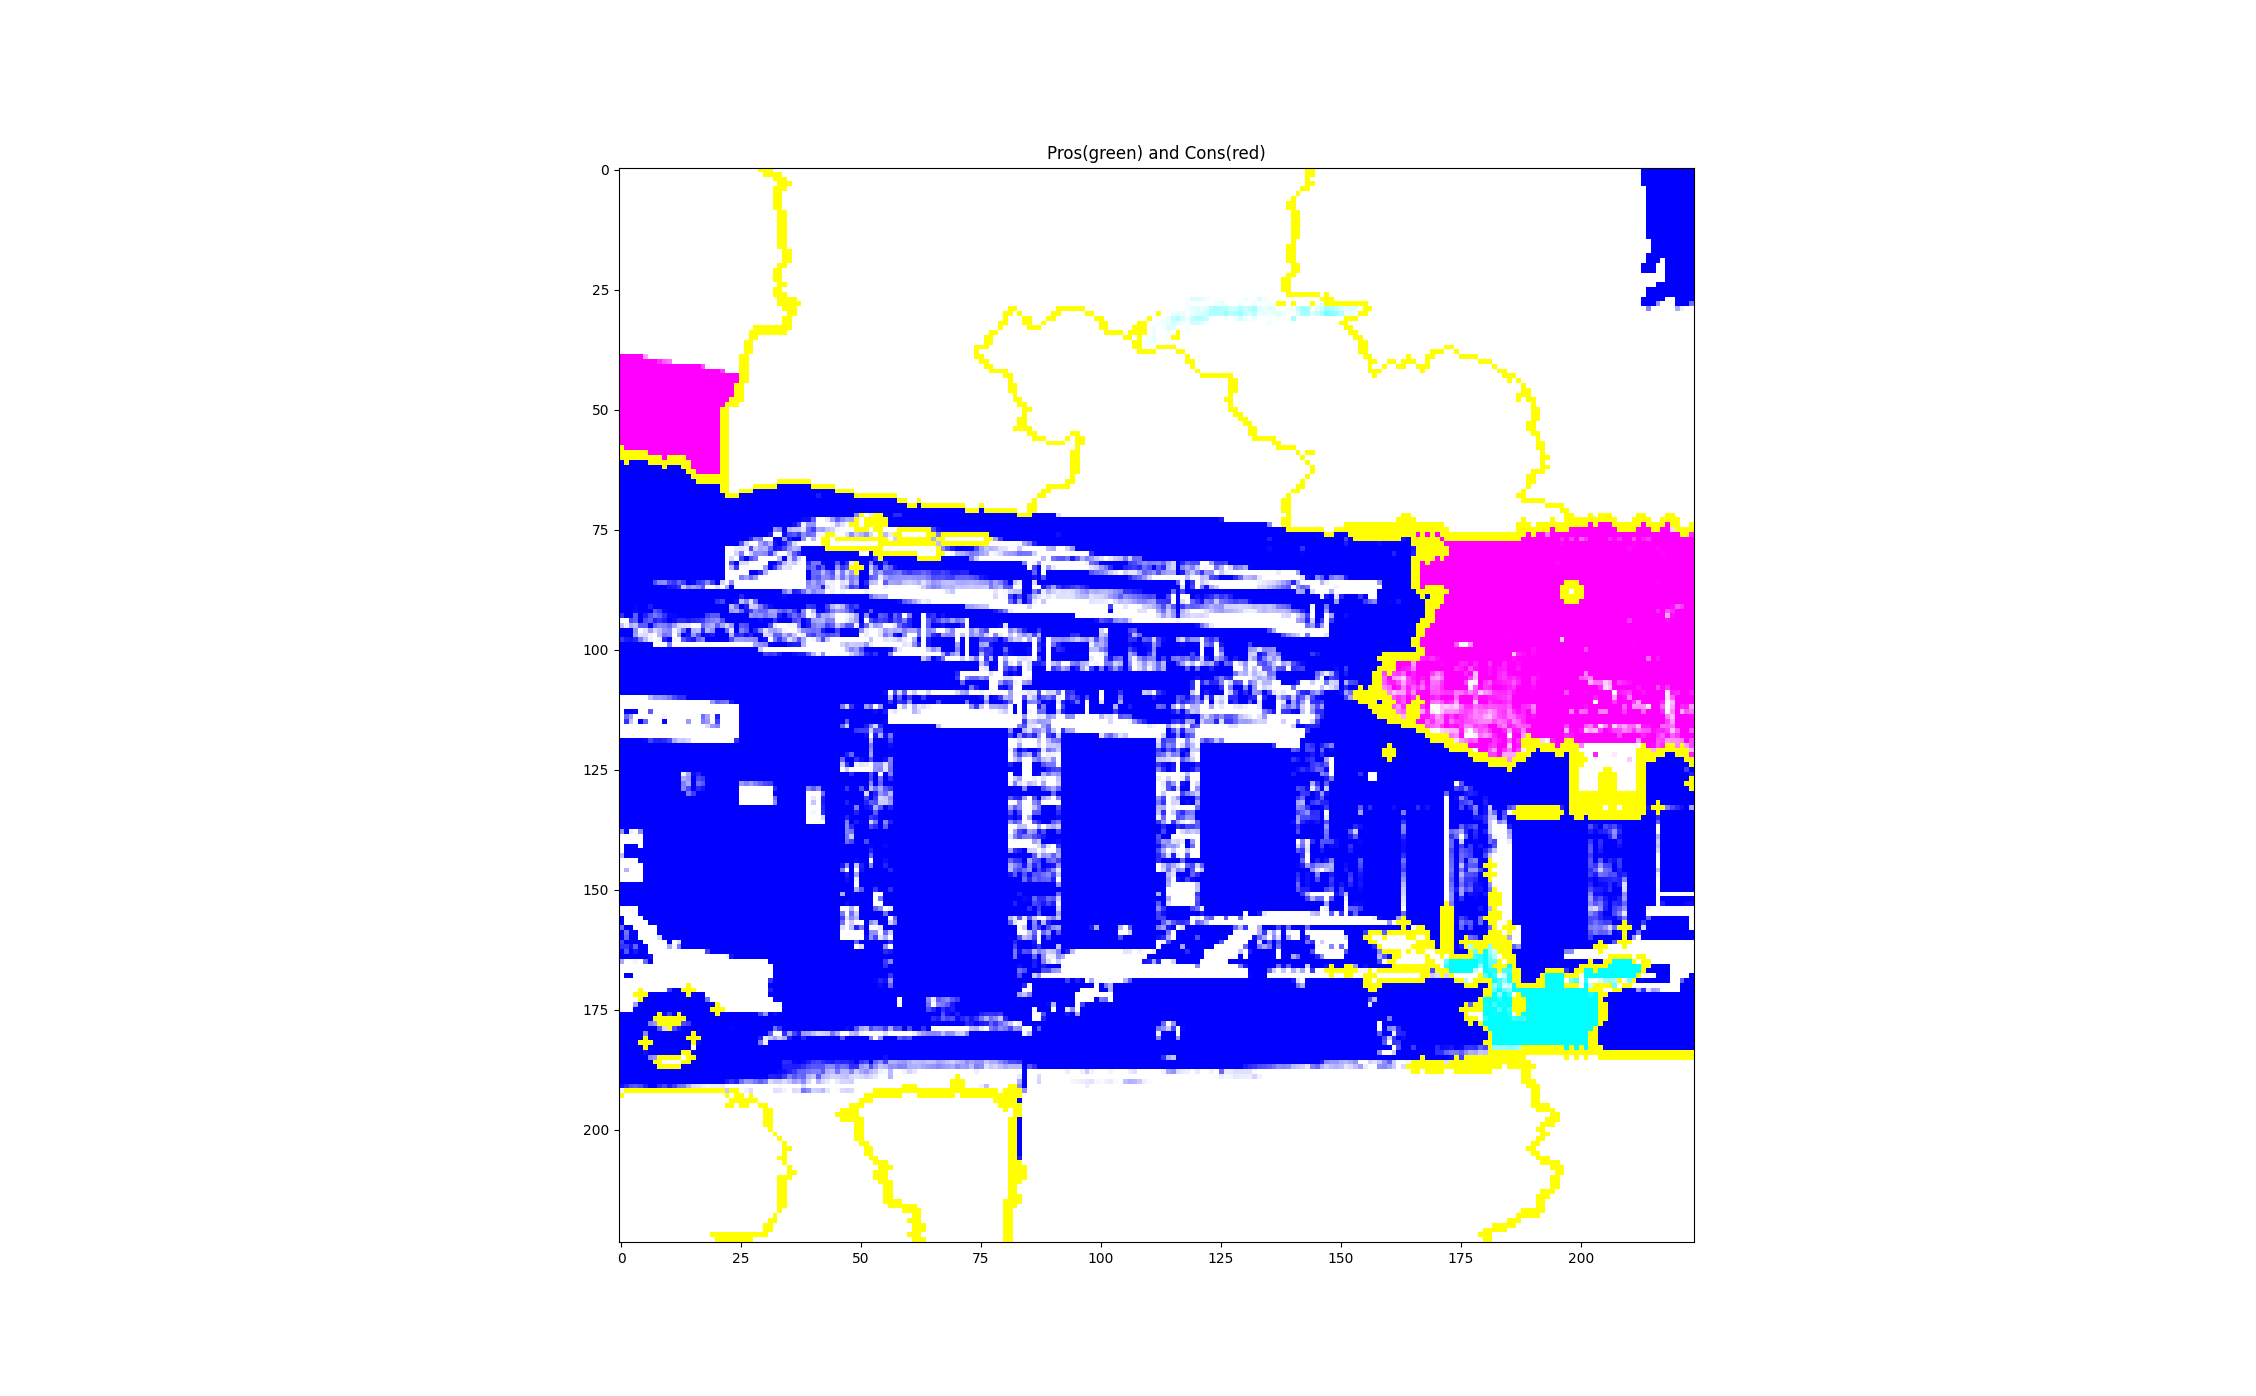
\includegraphics[width=7cm]{procon-suburb-should-insidecity.png}
    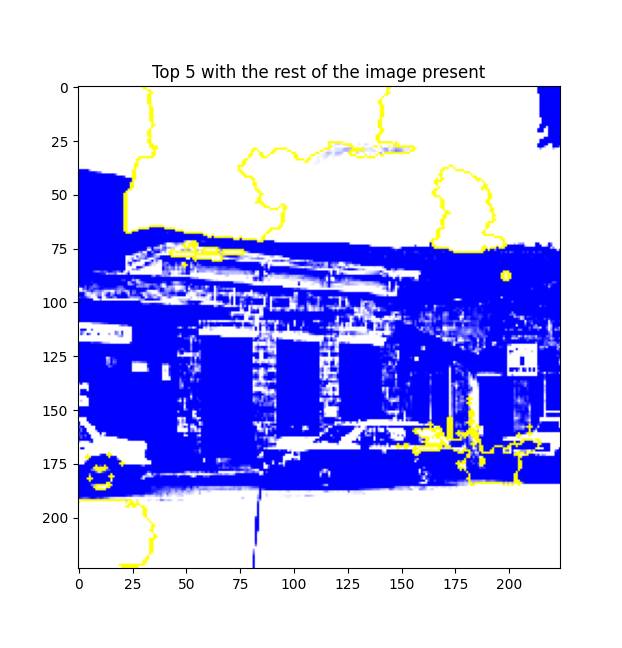
\includegraphics[width=7cm]{top5-suburb-should-inside-city.png}
    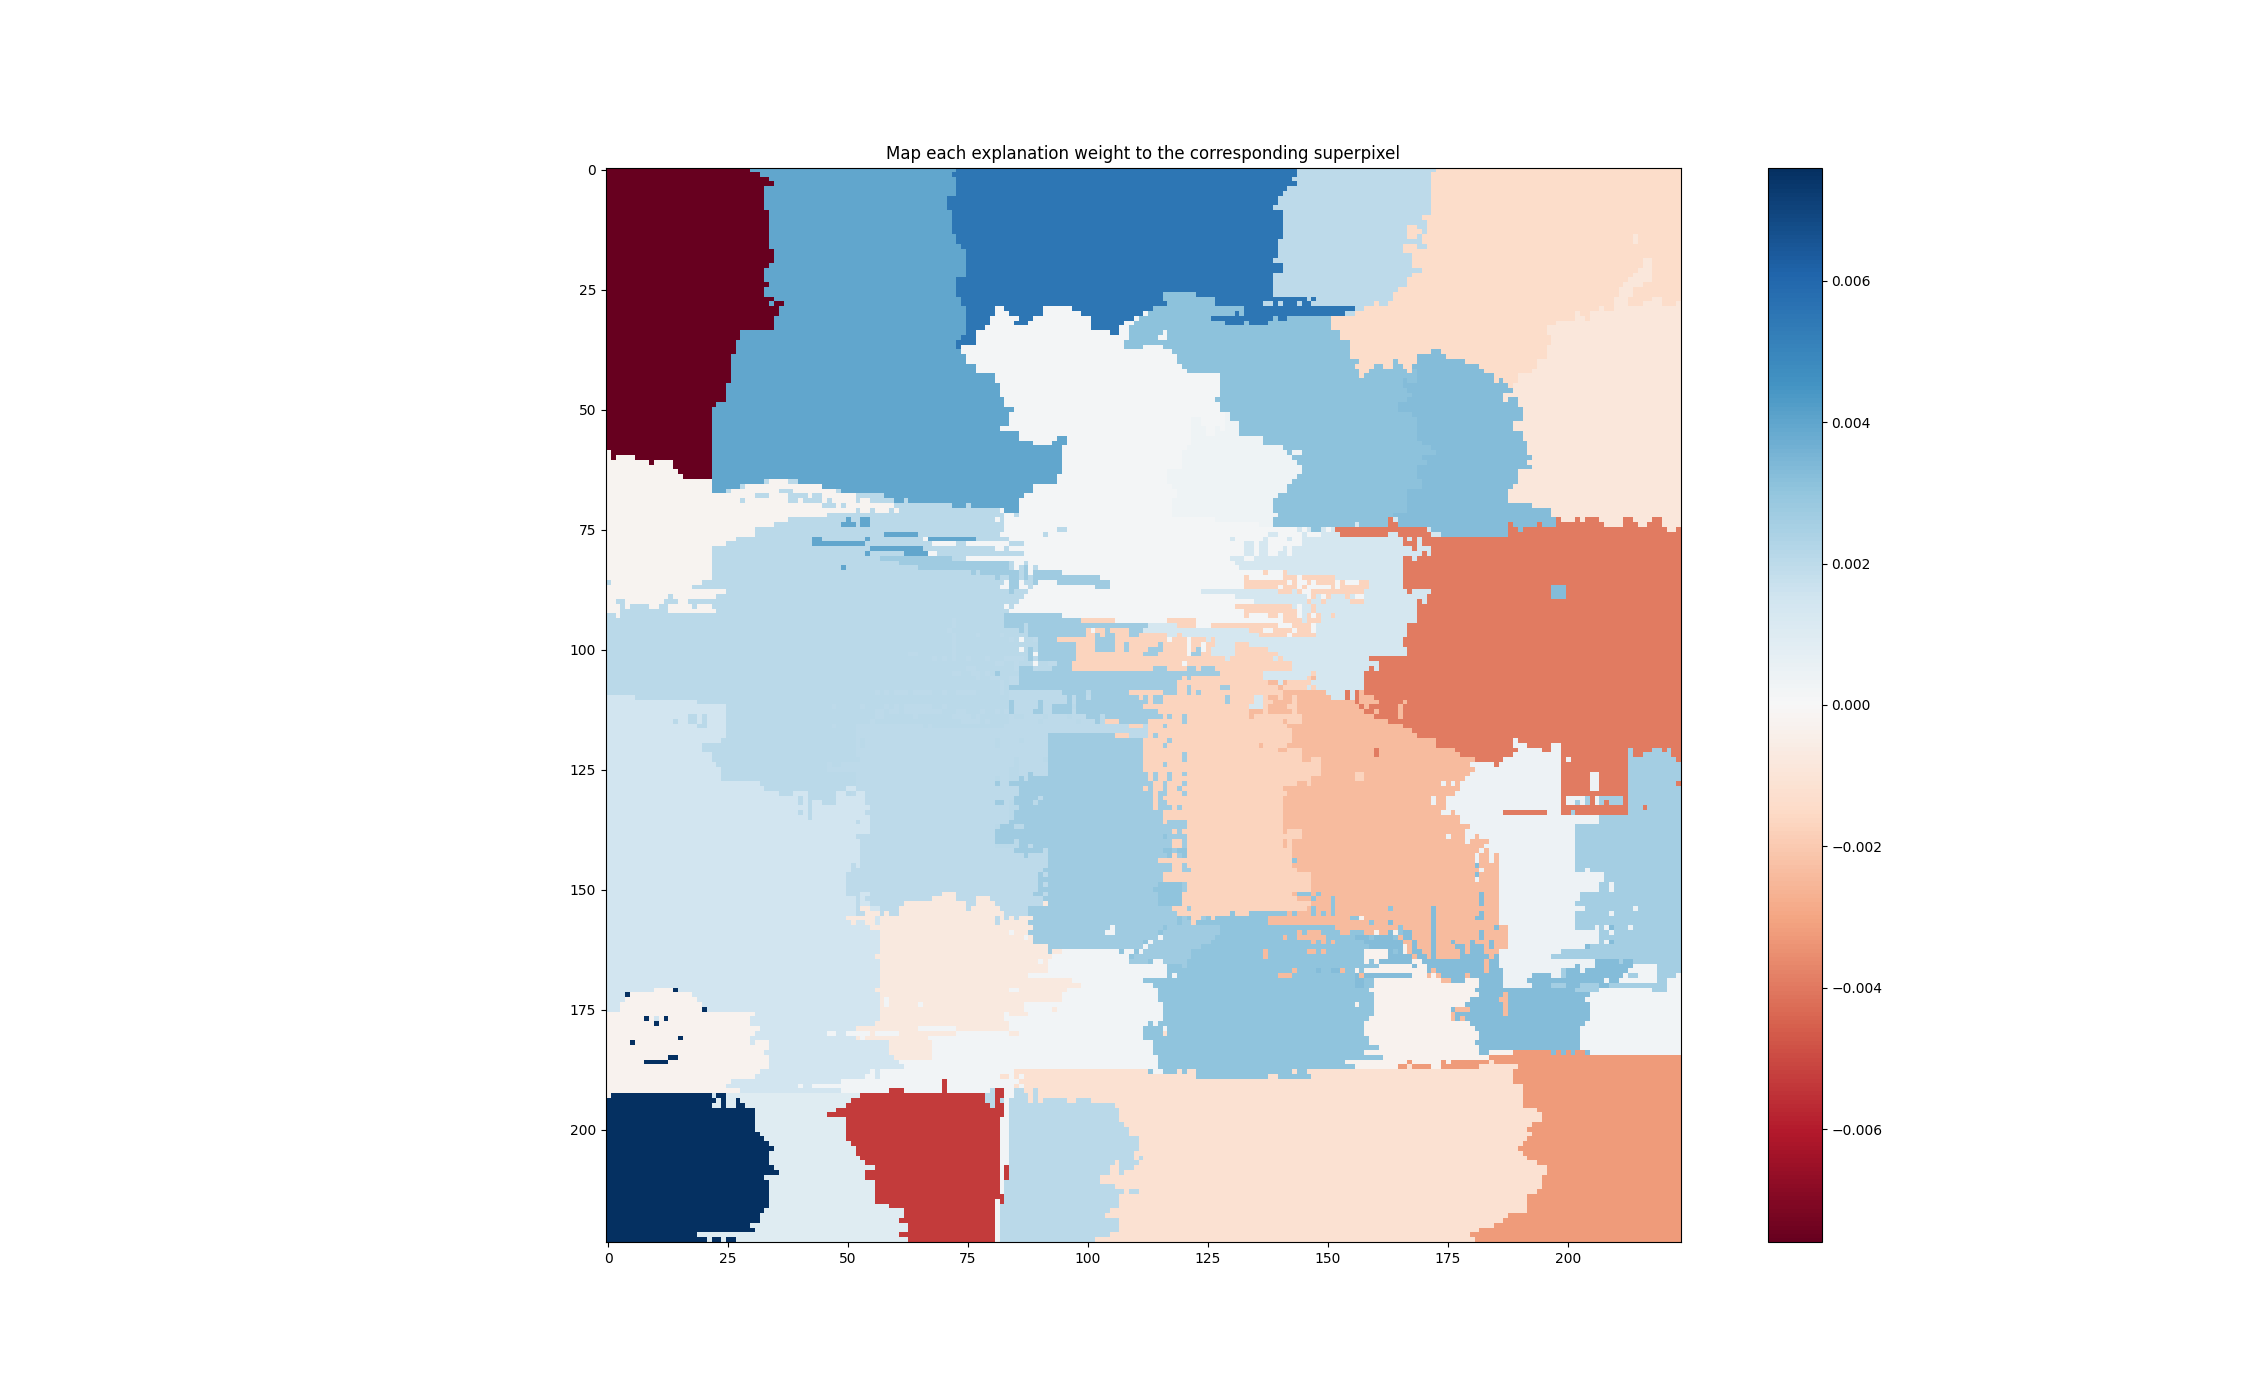
\includegraphics[width=7cm]{weight-suburb-should-insidecity.png}
    \caption{This is an inside city, but was predicted as a suburb.  Curious. It
    seems like the model didn't really care about the architecture. Instead it
    focused on the sky and the front of a car, and part of the street. It would
    make sense that it would confuse an outdoor image of a suburb with a city if
    it was just looking at the sky. }
    \label{fig:result1}
\end{figure}

\begin{figure}[H]
    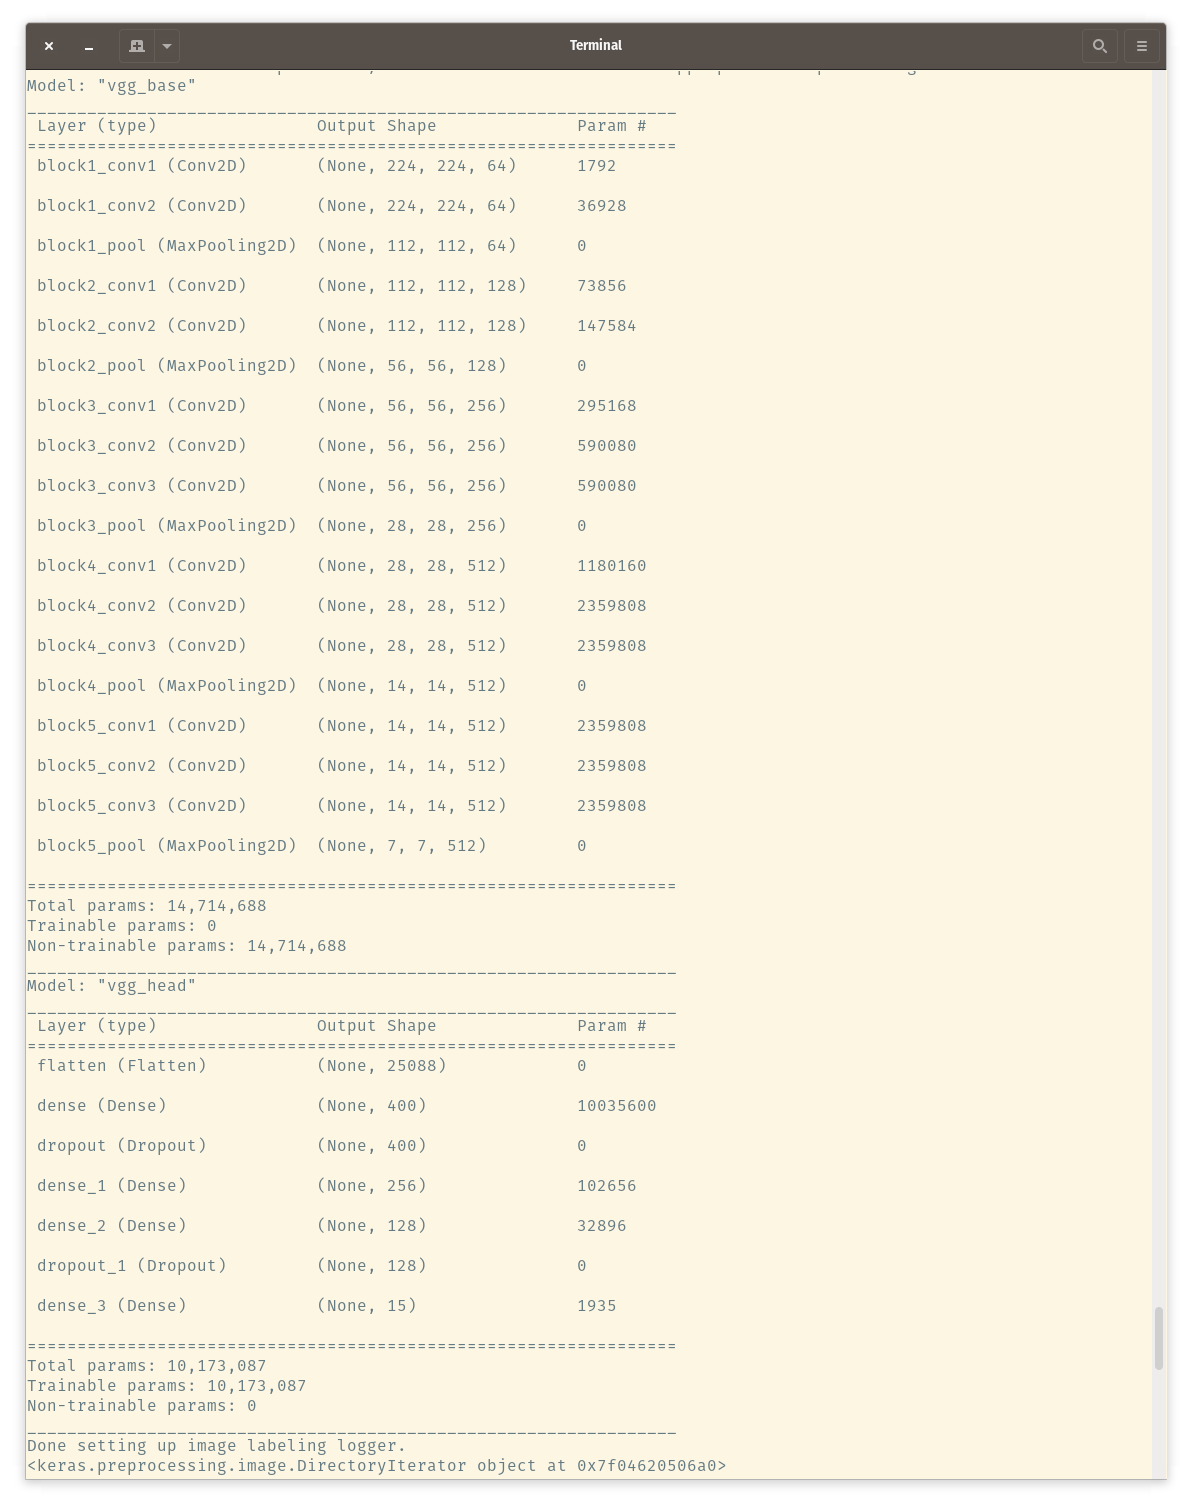
\includegraphics[width=10cm]{vgg-parameters.png}
    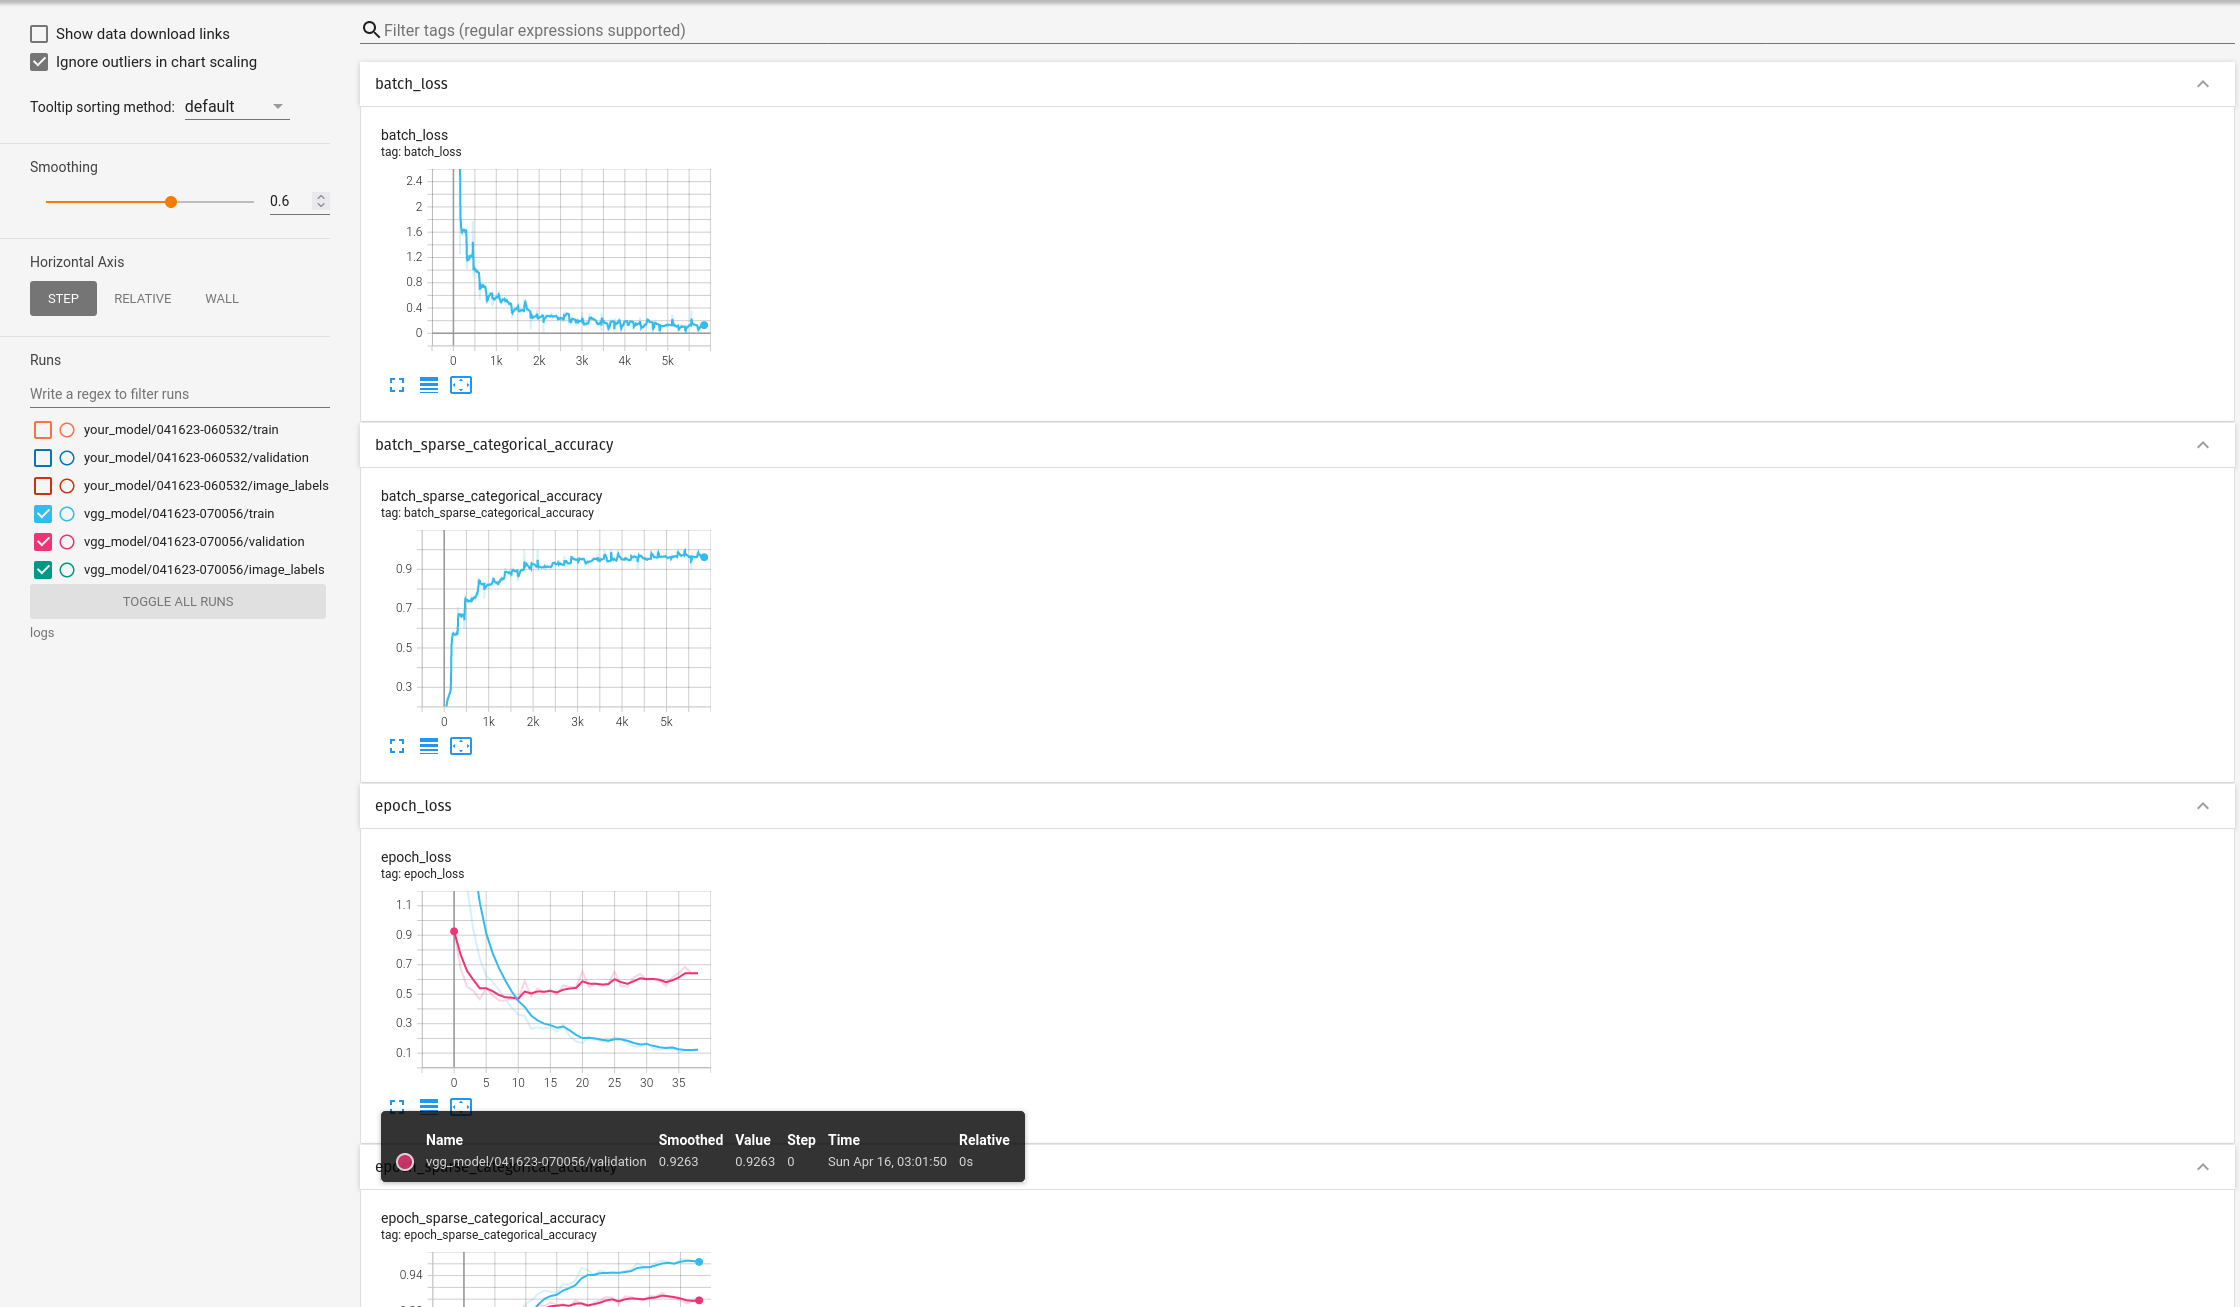
\includegraphics[width=10cm]{vgg-a.png}
    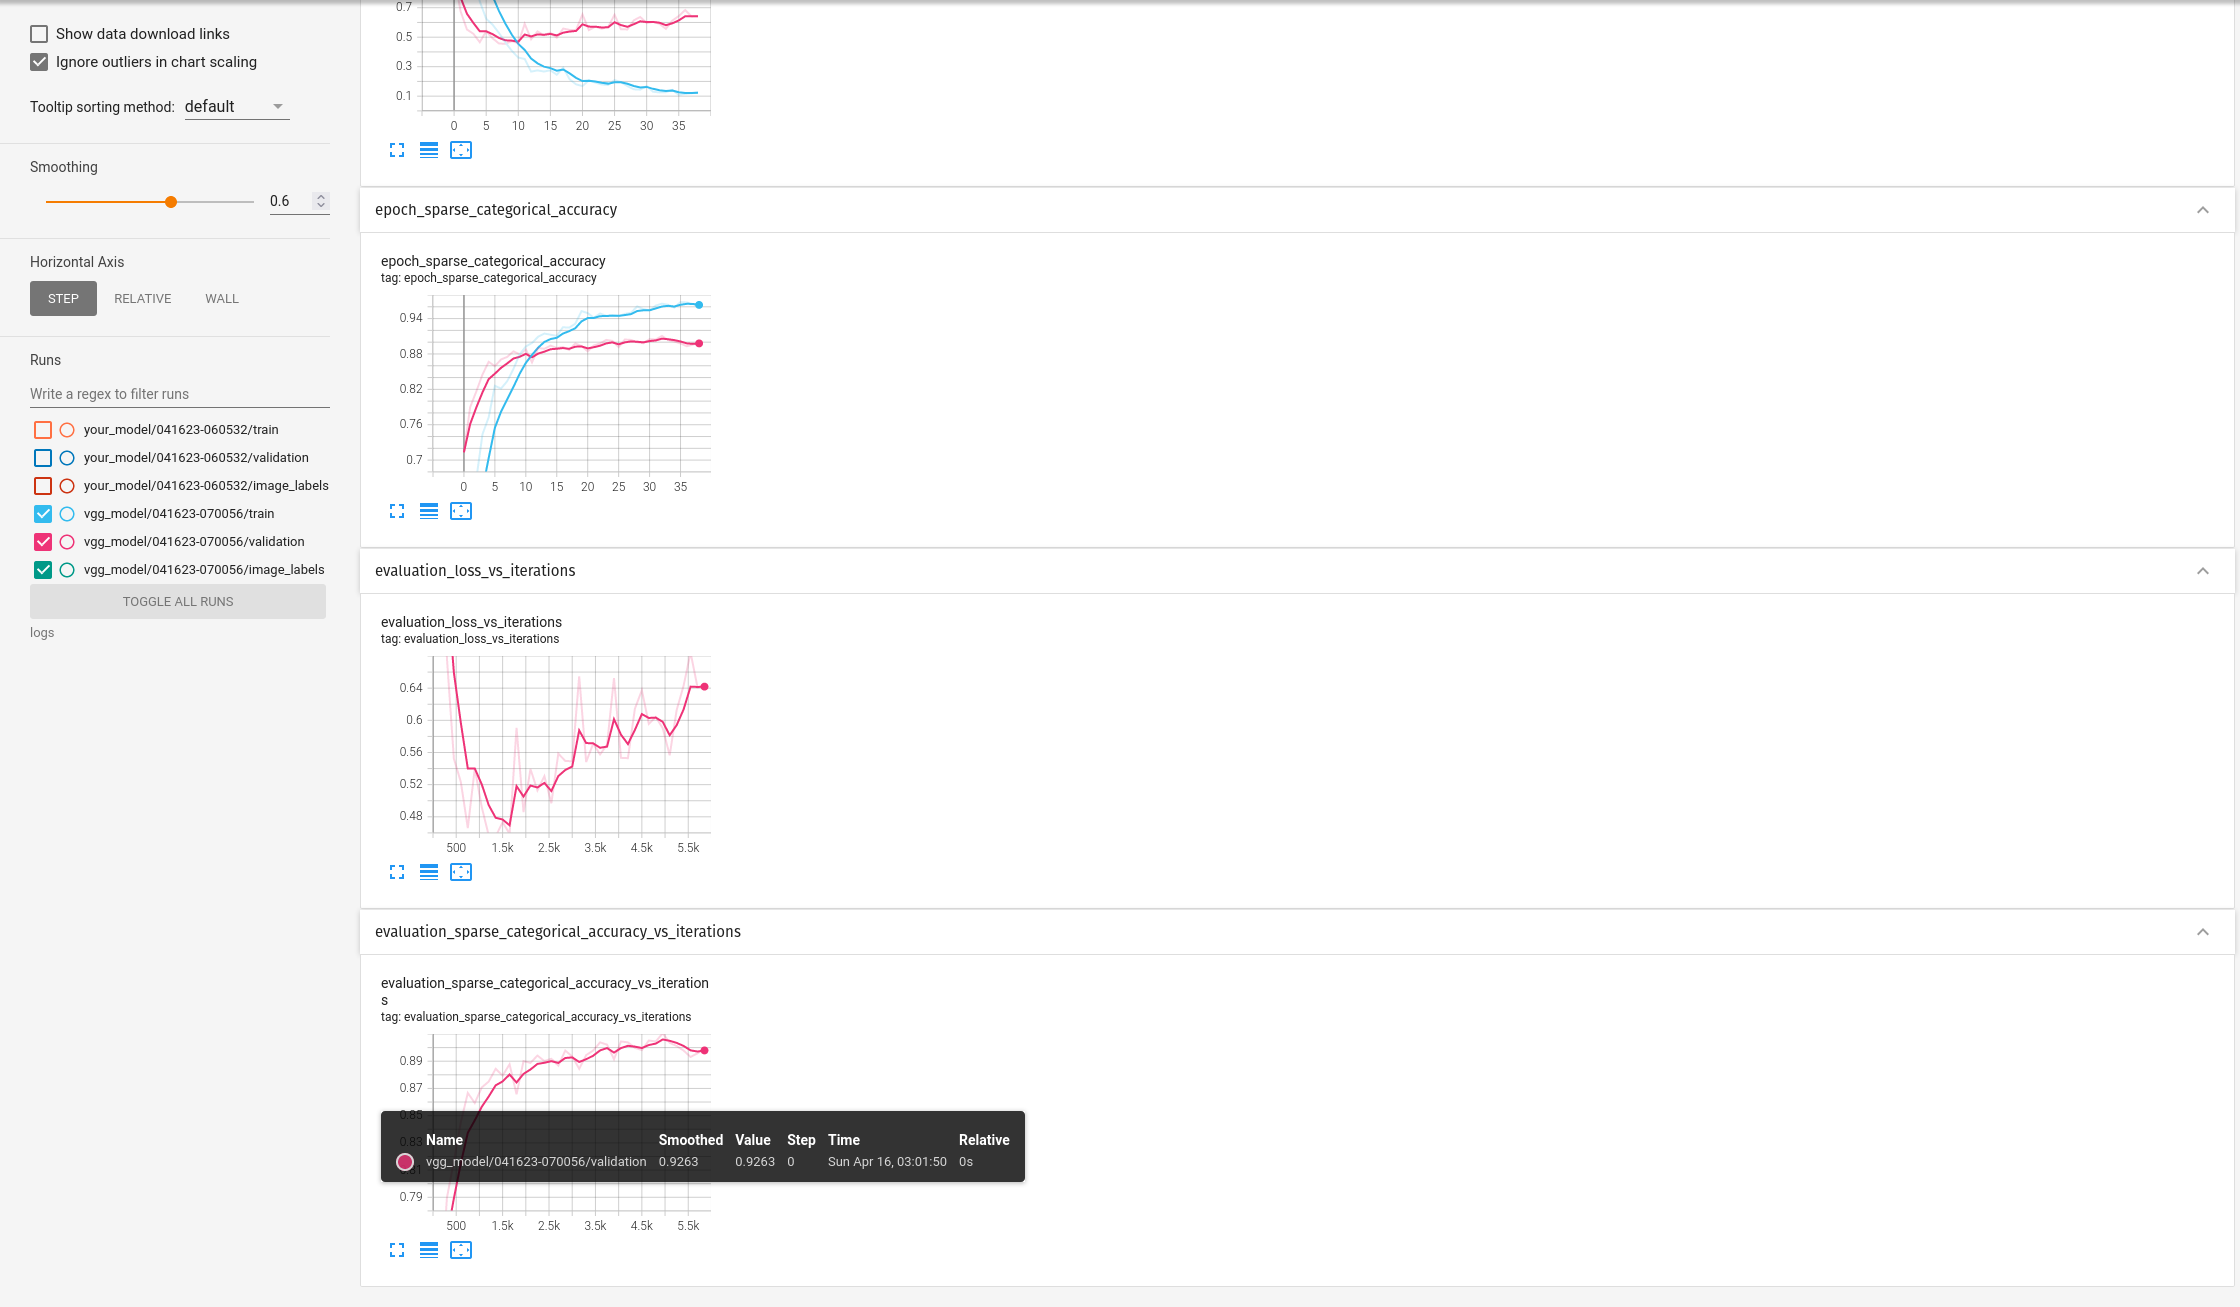
\includegraphics[width=10cm]{vgg-b.png}
    \caption{Task 3: Progress training head of the vgg model.}
    \label{fig:result1}
\end{figure}


% TODO: explanation

\end{document}
